\documentclass{beamer}

\usepackage[applemac]{inputenc}
\usepackage{graphicx}
\usepackage{listings}
\usepackage{setspace}  
\usepackage{stmaryrd}
\usepackage{nameref}
\usepackage{multimedia}
\usepackage{pgfpages}
\usepackage{relsize}

\usetheme{Boadilla}
\usecolortheme{seahorse}
\useoutertheme{shadow}

\setbeamercovered{transparent}

\setbeamertemplate{footline}{
	\begin{beamercolorbox}[wd=0.5\textwidth,ht=3ex,dp=1.5ex,leftskip=.5em,rightskip=.5em]{author in head/foot}
		\usebeamerfont{author in head/foot}
		\insertframenumber /\inserttotalframenumber\hfill\insertshortauthor~- \insertinstitute
	\end{beamercolorbox}
	\vspace*{-4.5ex}\hspace*{0.5\textwidth}
	\begin{beamercolorbox}[wd=0.5\textwidth,ht=3ex,dp=1.5ex,left,leftskip=.5em]{title in head/foot}
		\usebeamerfont{title in head/foot}
		\insertshorttitle
	\end{beamercolorbox}
}

\newcommand{\eq}[1]{\begin{equation*}#1\end{equation*}}
\newcommand{\eqa}[1]{\begin{eqnarray*}#1\end{eqnarray*}}

\newcommand{\ident}{\thesection.\thesubsection}
\newcommand{\mysubsection}[1]{\subsection{#1}\label{\ident}}

\newcommand{\ftitle}{\frametitle{\nameref{\ident}}}

\newcommand{\geant}{G{\smaller EANT}4 }
\newcommand{\geantws}{G{\smaller EANT}4}

\title[Flint - A tool for beamline design]{Integrating Tracking and Beam-Matter Interaction for Medical Beam Lines}
\subtitle{Dresden E{\smaller NLITE} 09}
\author{Lucas Clemente}
\institute{FZD, Dresden}
\date{April 3$^{\text{rd}}$ 2009}

\begin{document}

\begin{frame}
	\titlepage
\end{frame} 

\section{Introduction}

\mysubsection{The General Particle Tracer (GPT)}

\begin{frame}
	\ftitle
	\begin{columns}
		\begin{column}{6cm}
			\begin{block}{GPT}
				\begin{itemize}
					\item "A 3D code for accelerator and beamline design"
					\item Developed for 12 years (in C)
					\item Sophisticated tracking algorithm
					\item Good space-charge and multiple particle tracing
					\item Big repository of elements accessible
				\end{itemize}
			\end{block}
		\end{column}
		\begin{column}{5cm}
			\begin{figure}
				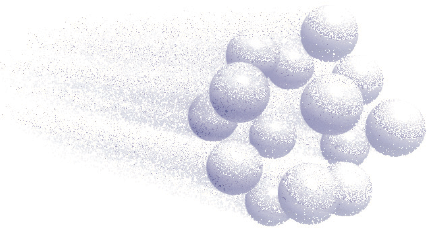
\includegraphics[width=0.7\columnwidth]{img/gpt}\vskip 0.5cm
				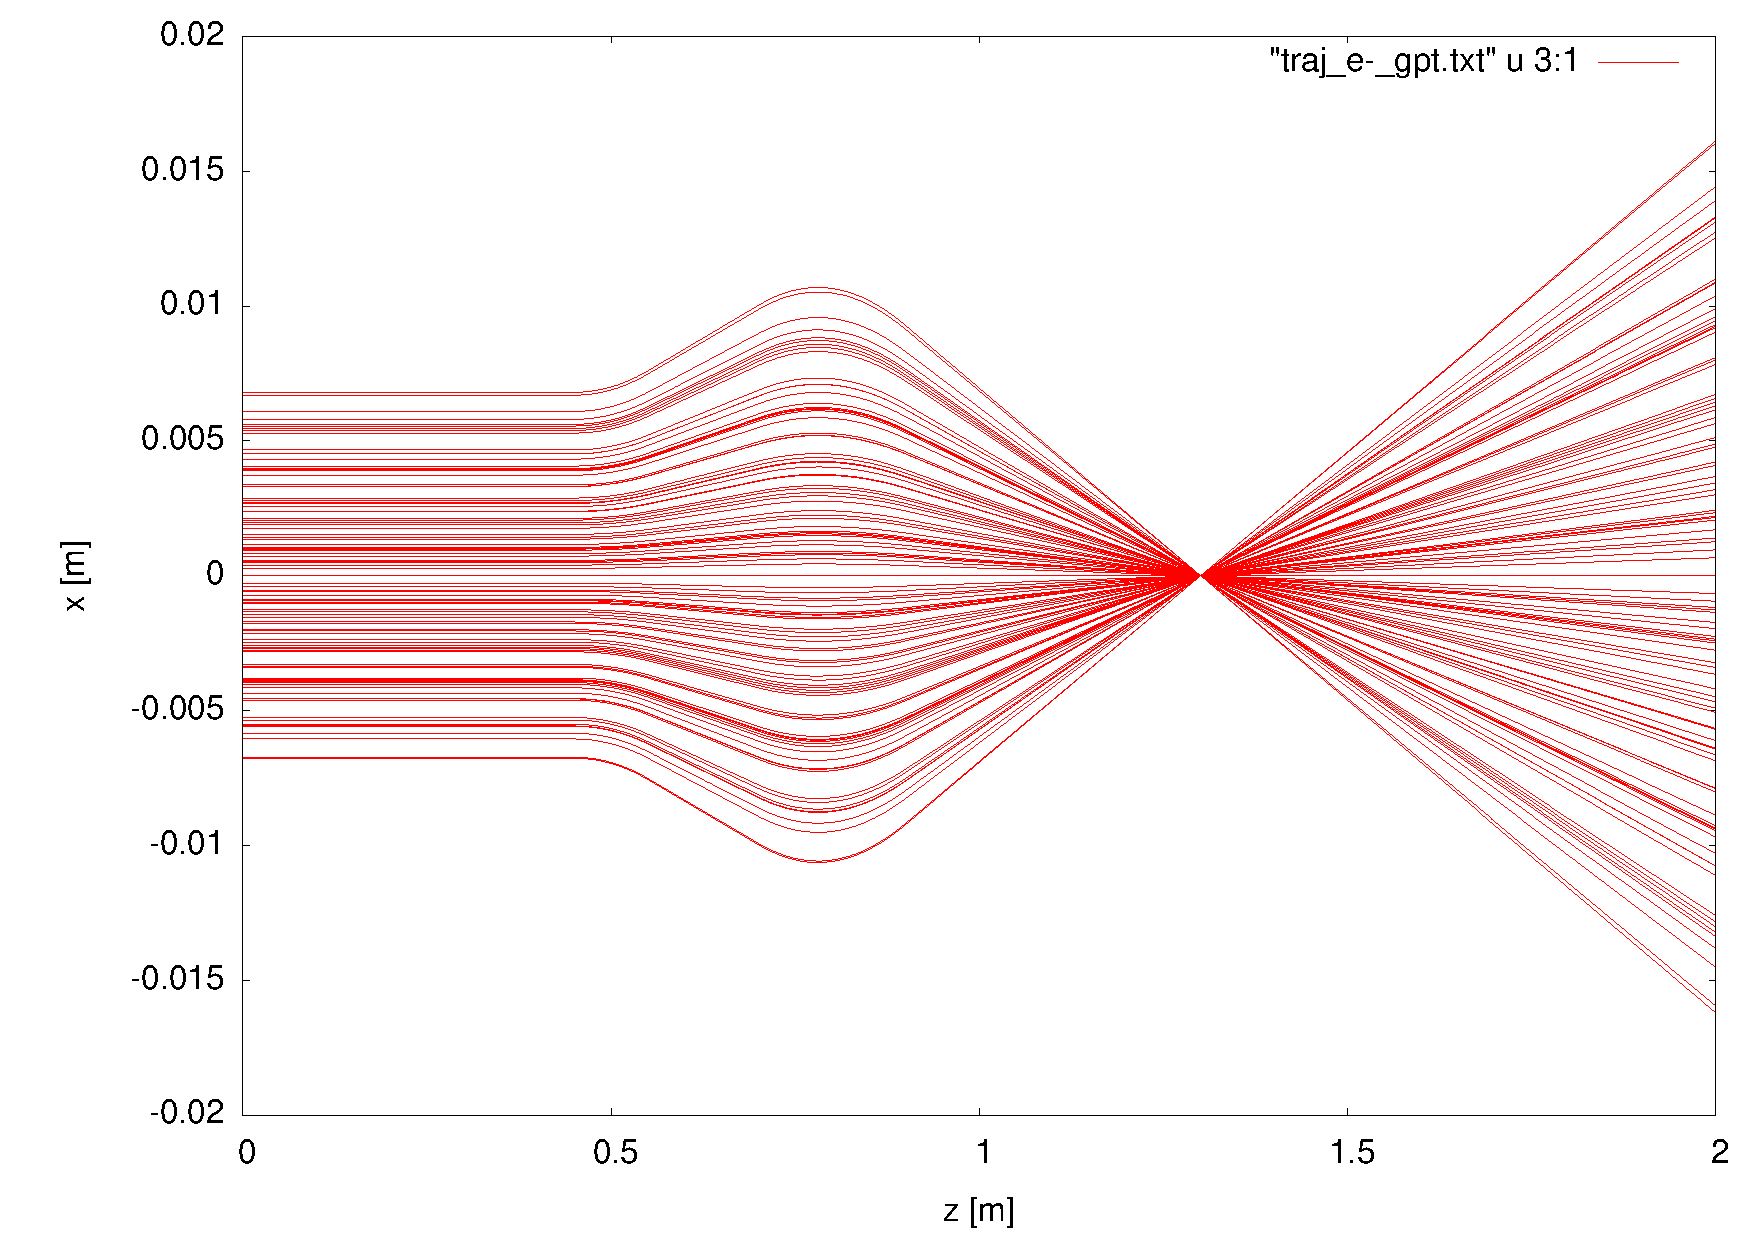
\includegraphics[width=\columnwidth]{img/quadrupole_gpt}
			\end{figure}
		\end{column}
	\end{columns}
\end{frame}

\begin{frame}
	\ftitle
	\begin{block}{How does it work?}
		\begin{itemize}
			\item $5^{th}$ order Runge-Kutta algorithm
			\item Stepwise tracking of \emph{multiple} particles through user-defined fields
			\item User interference possible using "custom elements"
			\item User may specify field components ($\vec{E}$, $\vec{B}$)
			\item No random but reproducable trajectories of \emph{real} particles
		\end{itemize}
	\end{block}
	\pause
	\begin{alertblock}{A Problem}
		Little to no particle matter interaction possible
	\end{alertblock}

\end{frame}

\begin{frame}
	\ftitle
	\begin{figure}
		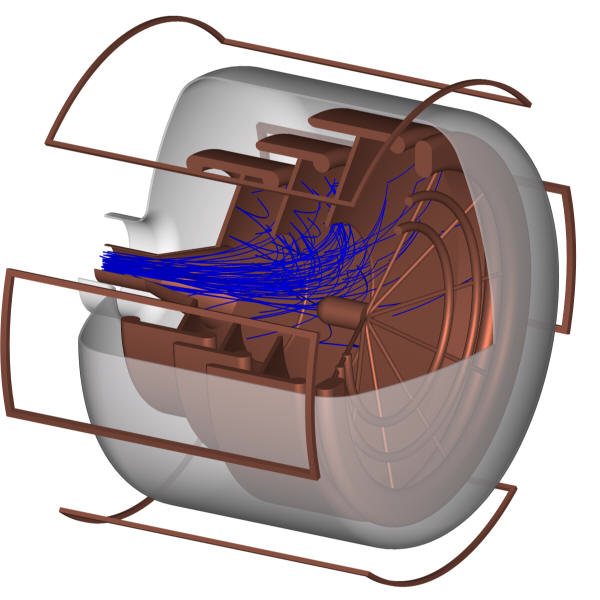
\includegraphics[height=0.7\textheight]{img/collector}
	\end{figure}
\end{frame}

\mysubsection{\geant}

\begin{frame}
	\ftitle
	\begin{columns}
		\begin{column}{6cm}
			\begin{block}{\textbf{GE}ometry \textbf{AN}d \textbf{T}racking 4}
				\begin{itemize}
					\item Toolkit for the simulation of particle-matter interactions
					\item Developed for 15 years at CERN (C++)
					\item Advanced geometry system
					\item Proofed correct in many experiments
				\end{itemize}
			\end{block}
		\end{column}
		\begin{column}{5cm}
			\begin{figure}
				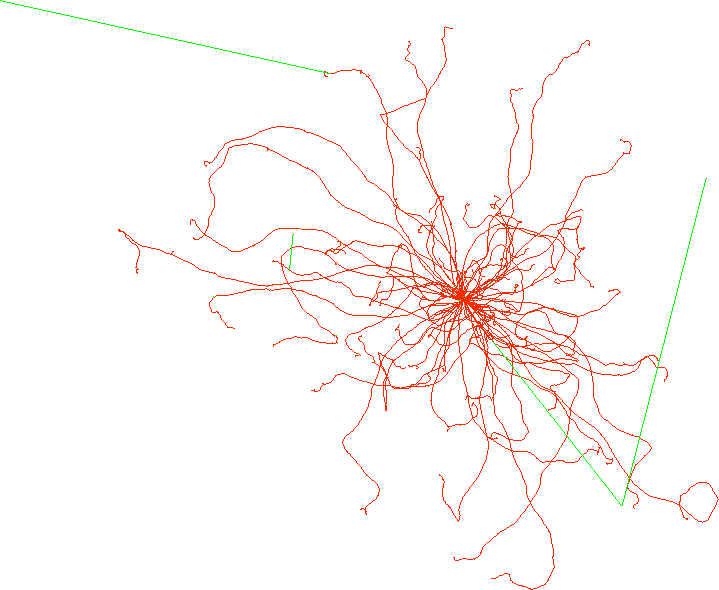
\includegraphics[width=0.55\columnwidth]{img/geant_e}\vskip 0.5cm
				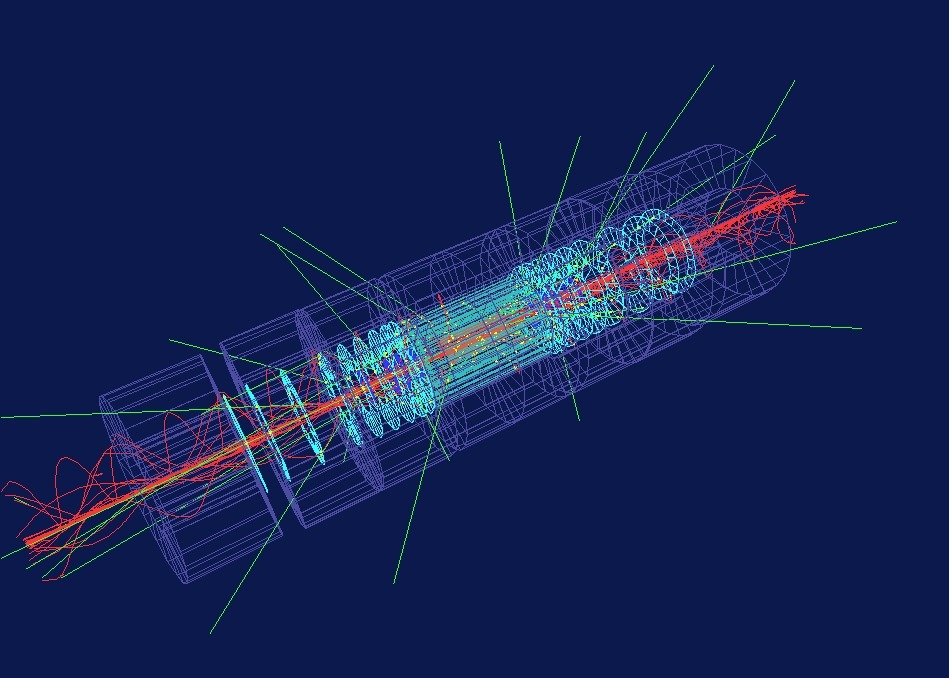
\includegraphics[width=0.95\columnwidth]{img/atlas}
			\end{figure}
		\end{column}
	\end{columns}
\end{frame}

\begin{frame}
	\ftitle
	\begin{block}{How does it work?}
		\begin{itemize}
			\item Monte-Carlo algorithm
			\item Stepwise tracking of \emph{single} particles through user-defined geometries
			\item User can overload nearly any class or supply his own (Open-source)
			\item Random particle trajectories, statistical simulation of \emph{Monte-Carlo particles}
		\end{itemize}
	\end{block}
	\pause
	\begin{alertblock}{Some Problems}
		\begin{itemize}
			\item Only single-particle simulations possible (no space charge, ...)
			\item Modest electromagnetic fields
		\end{itemize}
	\end{alertblock}
\end{frame}

\mysubsection{Challenges of a beamline modelling software}

\begin{frame}
	\ftitle
	\begin{block}{Medical beamlines}
		\begin{itemize}
			\item Compact proton / ion sources require a compact beamline
			\item Scaling of beamlines not possible
			\item Radiation protection!
		\end{itemize}
	\end{block}
	\pause
	\begin{alertblock}{State of the art}
		\begin{center}
			There is no code combining advanced tracking and particle-matter interactions!
		\end{center}
	\end{alertblock}
\end{frame}

\section{Flint in general}

\mysubsection{What is Flint?}

\begin{frame}
	\ftitle
	\begin{block}{\textbf{F}ZD \textbf{L}aser \textbf{In}teractor and \textbf{T}racker}
			A simulation software fundamentally combining GPT and \geant
	\end{block}
	\pause
	\begin{exampleblock}{Features}
		\begin{itemize}
			\item Tracking massive amounts of particles through complex geometries
			\item All of GPT's space charge algorithms
			\item Full \geant capabilities in particle-matter interaction
			\item All geometry elements and fields of GPT and \geant
			\item Customizability
			\item High-Speed due to parallelization using OpenMP
		\end{itemize}
	\end{exampleblock}
\end{frame}

\begin{frame}
	\frametitle{A simple calculation using GPT...}
	\begin{figure}
		\begin{center}
			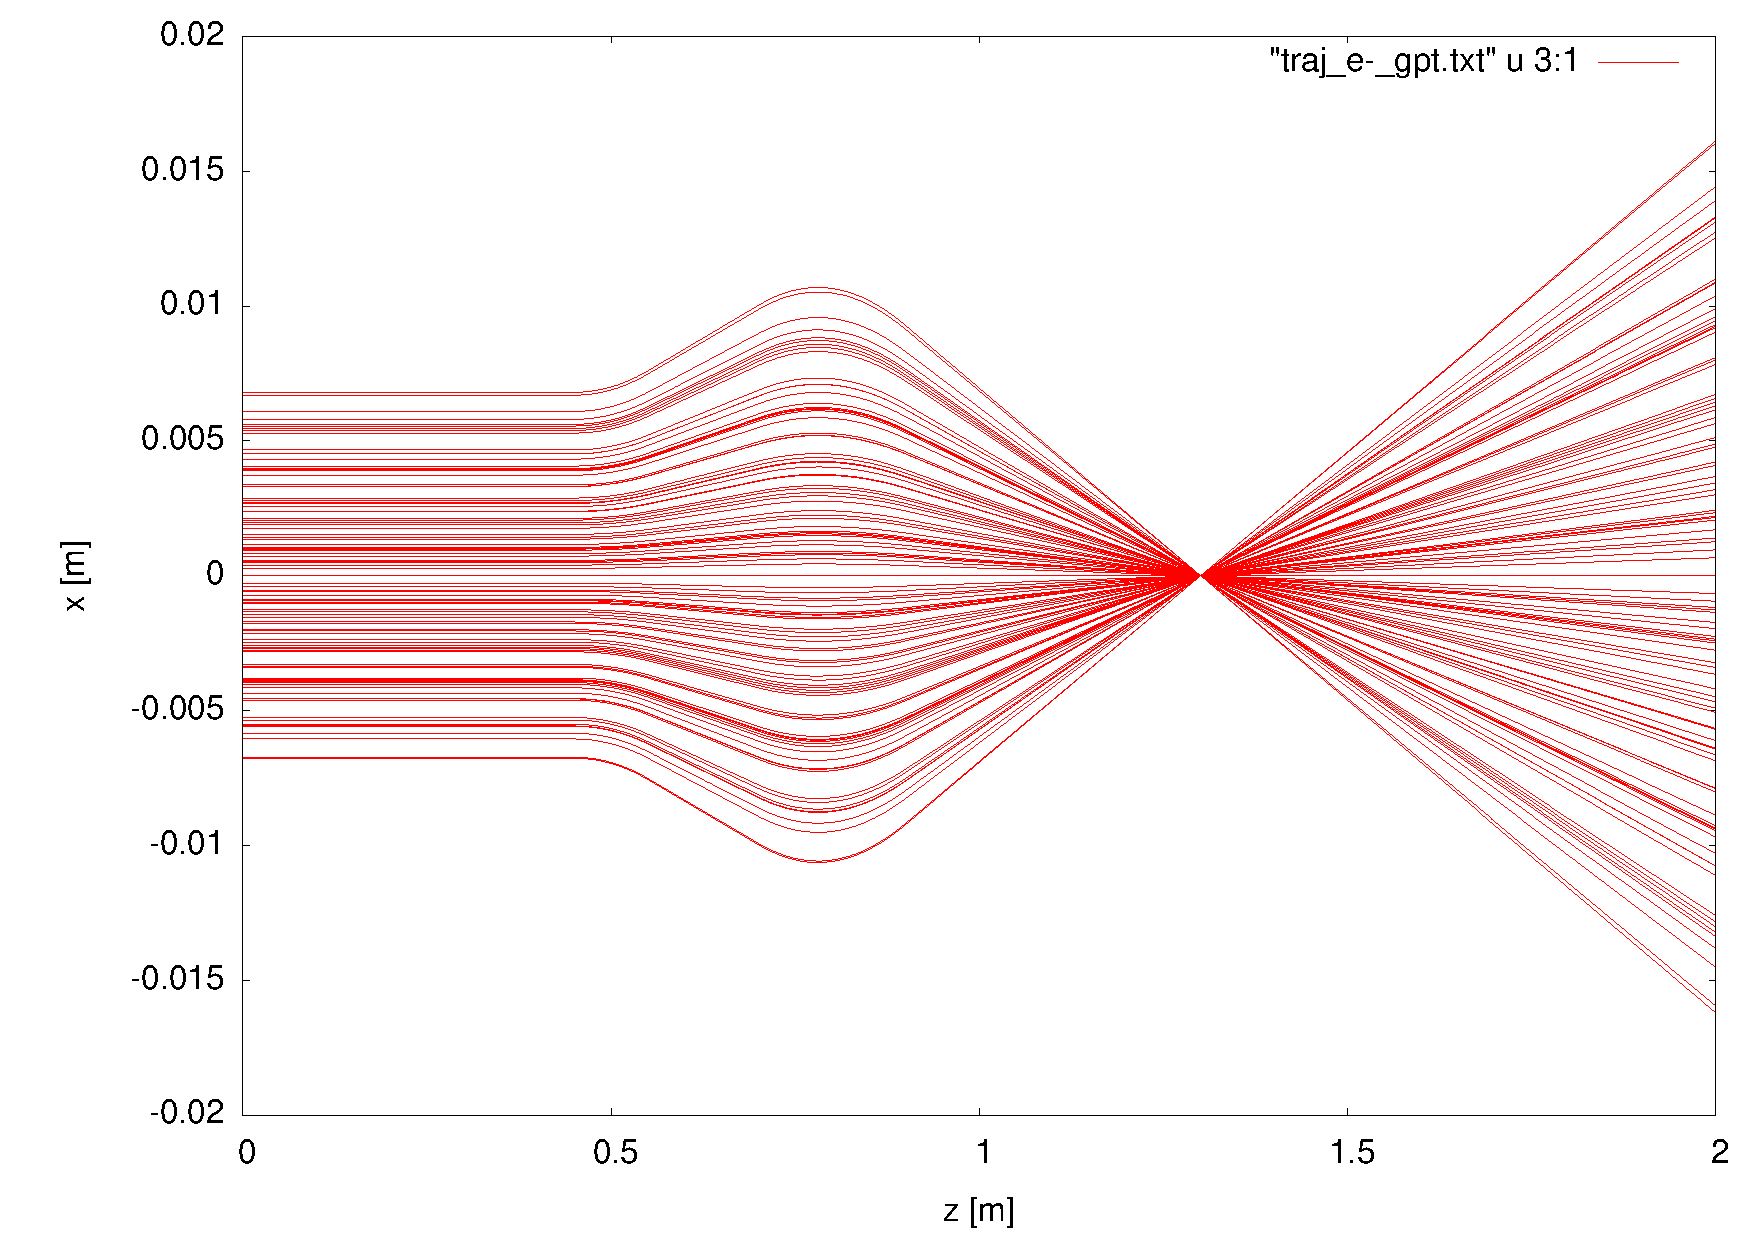
\includegraphics[height=0.7\textheight]{img/quadrupole_gpt}
			\caption{Electron beam ($\gamma = 100$) passing through two quadrupoles ($G = 3.9, -3.25 ~\frac{T}{m}$)}
		\end{center}
	\end{figure}
\end{frame}

\begin{frame}
	\frametitle{... and Flint}
	\begin{figure}
		\begin{center}
			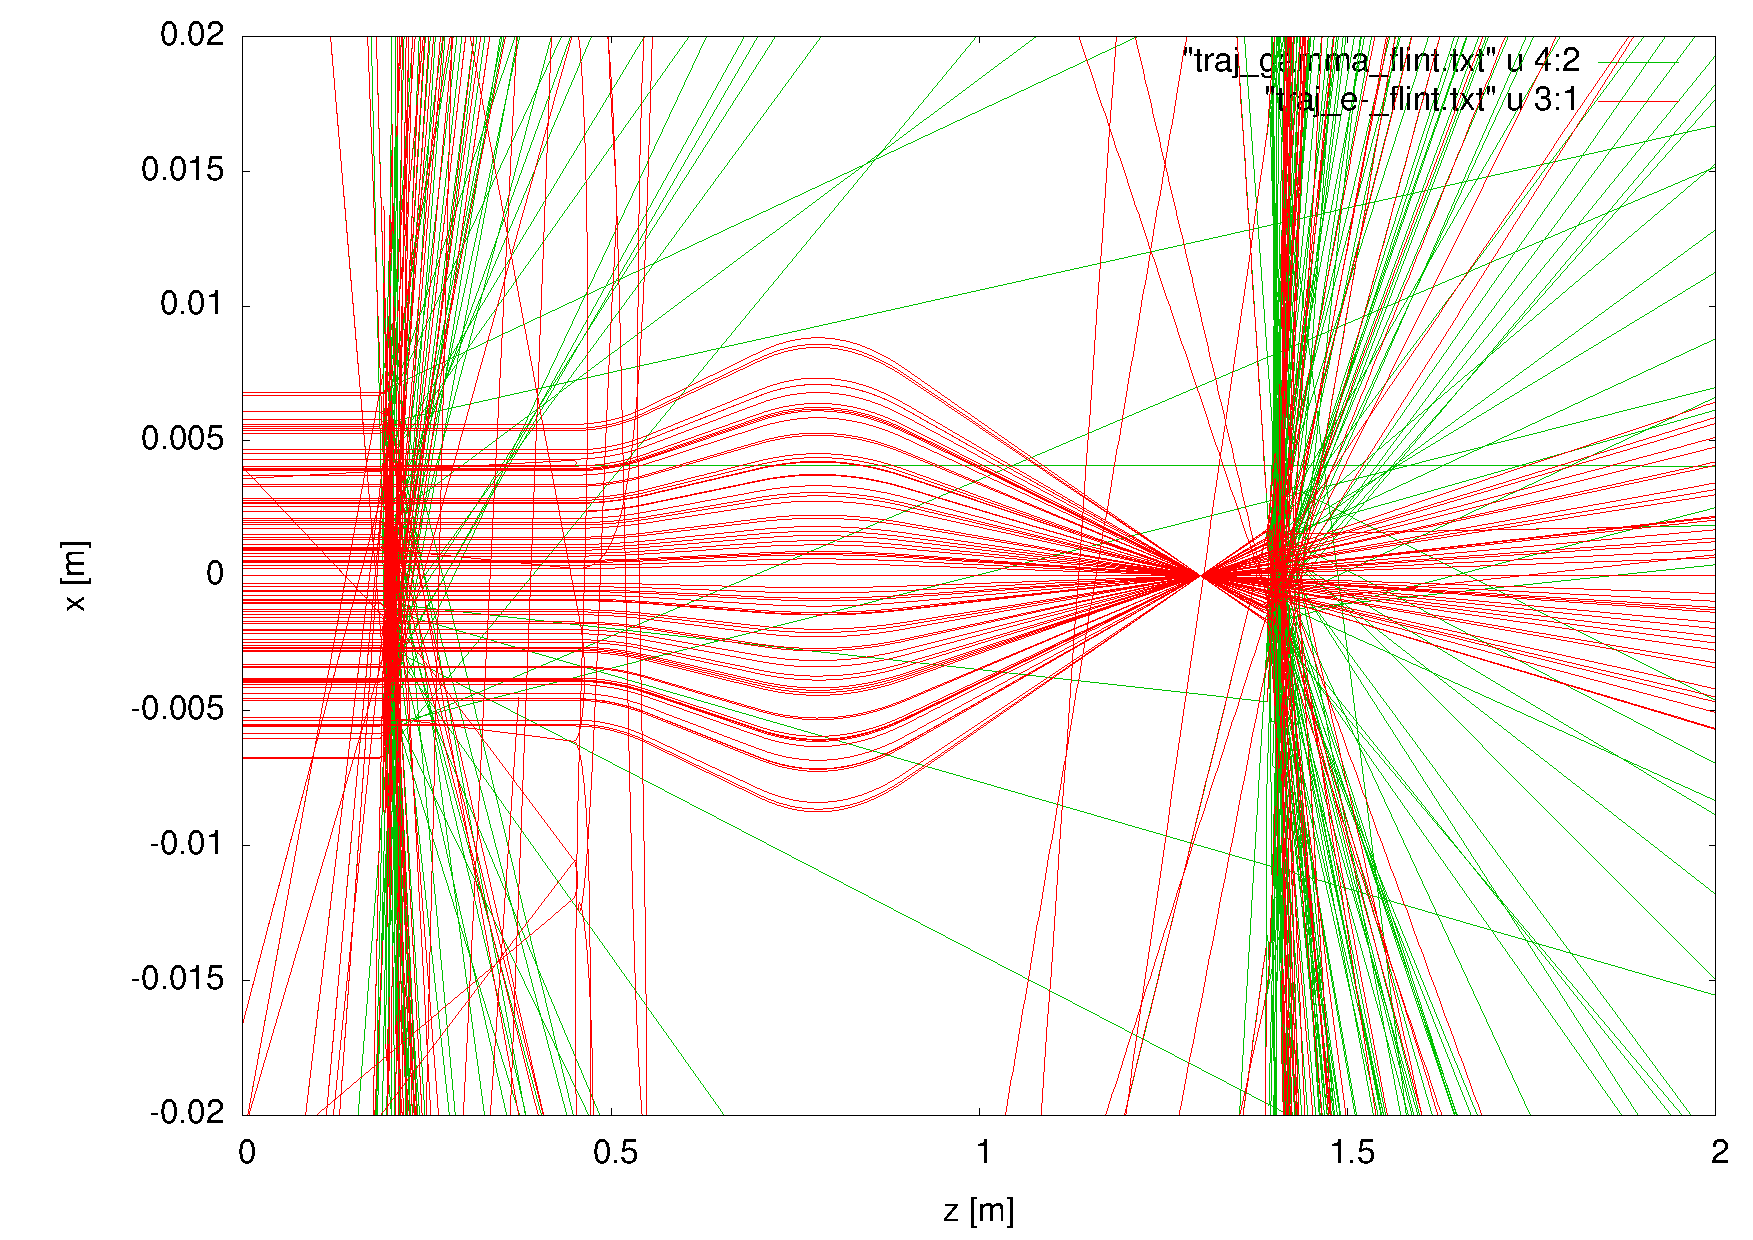
\includegraphics[height=0.7\textheight]{img/quadrupole_flint}
			\caption{Electron beam ($\gamma = 100$) passing through two quadrupoles ($G = 3.9, -3.25 ~\frac{T}{m}$) and two pinholes ($Cu$, $dz = 2~cm$)}
		\end{center}
	\end{figure}
\end{frame}

\mysubsection{Architecture}

\begin{frame}
	\ftitle
	\begin{block}{How is it built?}
		\begin{itemize}
			\item Problem: GPT only limited extendable\\
				$\Rightarrow$ Custom field elements
			\item GPT is C, \geant is C++
			\item Solution: Link a \geant based library
			\item Other used libraries:
				\begin{itemize}
					\item xerces for XML-configuration
					\item CLHEP
					\item OpenMP (included in gcc4)
				\end{itemize}
		\end{itemize}
	\end{block}
	\pause
	\begin{exampleblock}{What is flint?}
		Flint consists of a \geant based library to be linked into GPT, a GPT custom element and a bunch of tools for modelling, run and analysis.
	\end{exampleblock}
\end{frame}

\begin{frame}
	\ftitle
	\begin{block}{The element ``G4Virtual''}
		Include \geant just by typing\\
		\texttt{G4Virtual("WCS", "I");}
	\end{block}
	\pause
	\begin{exampleblock}{Program flow}
		\begin{itemize}
			\item Calculate normal GPT step
			\item After each succesful step do for each particle:
				\begin{itemize}
					\item Check for intersection with a \geant solid (pre and post step point)
					\item Use \geant for recalculation of the step
					\item Inject the results of \geant into GPT
					\item Output the particle's data (e.g. trajectories, dose)
				\end{itemize}
		\end{itemize}
	\end{exampleblock}
\end{frame}


\mysubsection{Combined Stepping}

\begin{frame}
	\ftitle
	\begin{columns}
		\begin{column}{7.5cm}
			\begin{block}{A step in Flint}
				\begin{enumerate}[<alert@+>]
					\item Use GPT to track the step
					\item Recalculate the step using \geant\\
						\begin{itemize}
							\item Start at pre-GPT-point
							\item Track in direction of post-GPT point
							\item Stop when time exceeds the GPT time
						\end{itemize}
					\item Inject the results of \geant into GPT\\
						\begin{itemize}
							\item Take the new position and velocities
							\item Calculate the rotation of momentum between pre-\geant and post-\geant
							\item Rotate the post-GPT momentum accordingly
						\end{itemize}
				\end{enumerate}
			\end{block}
		\end{column}
		\begin{column}{3.5cm}
			\begin{exampleblock}{An example}
				\begin{figure}
					\only<1,2>{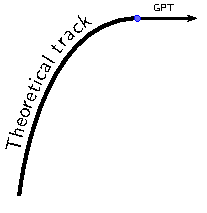
\includegraphics[width=\columnwidth,page=1]{img/stepping}}
					\only<3>{\includegraphics[width=\columnwidth,page=2]{img/stepping}}
					\only<4>{\includegraphics[width=\columnwidth,page=3]{img/stepping}}
					\only<5,6>{\includegraphics[width=\columnwidth,page=4]{img/stepping}}
					\only<7>{\includegraphics[width=\columnwidth,page=5]{img/stepping}}
					\only<8>{\includegraphics[width=\columnwidth,page=6]{img/stepping}\vskip 0pt~}
					\only<9>{\includegraphics[width=\columnwidth,page=7]{img/stepping}\vskip 0pt~}
				\end{figure}
			\end{exampleblock}
		\end{column}	
	\end{columns}
\end{frame}

\mysubsection{Secondaries}

\begin{frame}
	\ftitle
	\begin{block}{Secondary particles}
		\begin{itemize}
		 \item \geant produces all kind of secondaries
		 \item GPT can only handle massive and charged particles
		\end{itemize}
	\end{block}
	\pause
	\begin{exampleblock}{The solution}
		\begin{itemize}
			\item Massive and charged particles are injected into GPT
			\item Massless or chargeless particles are tracked \emph{and outputted} solely by \geant
		\end{itemize}
	\end{exampleblock}
\end{frame}

\section{Using Flint}

\mysubsection{Design of beamlines}

\begin{frame}
	\ftitle
	\begin{block}{Input}
		Only one input file (XML) consisting of:
		\begin{itemize}
			\item GDML part (\textbf{G}eometry \textbf{D}escription \textbf{M}arkup \textbf{L}anguage, supported naturally by \geantws)
			\item GPT part (In general GPT \texttt{ini} file)
			\item Some additional tags controlling Flint
		\end{itemize}
	\end{block}
	\pause
	\begin{exampleblock}{Example: Configuring particles used in \geant}
		\texttt{<particles>\\
			~~<particle name="gamma" />\\
			~~<particle name="e-" />\\
			~~<particle name="proton" />\\
			</particles>
		}
	\end{exampleblock}
\end{frame}

\begin{frame}
	\ftitle
	\begin{block}{Example: A pinhole}
		\texttt{<tube name="pinhole" z="20.0" rmin="10.0" rmax="100.0" />\\
			<volume name="pinhole">\\
			~~<materialref ref="Cu" />\\
			~~<solidref ref="pinhole" />\\
			</volume>\\
			<position name="ph" z="1400.0" />\\
			<physvol>\\
			~~<volumeref ref="pinhole" />\\
			~~<positionref ref="ph" />\\
			</physvol>
		}
	\end{block}
\end{frame}

\begin{frame}
	\ftitle
	\begin{figure}
		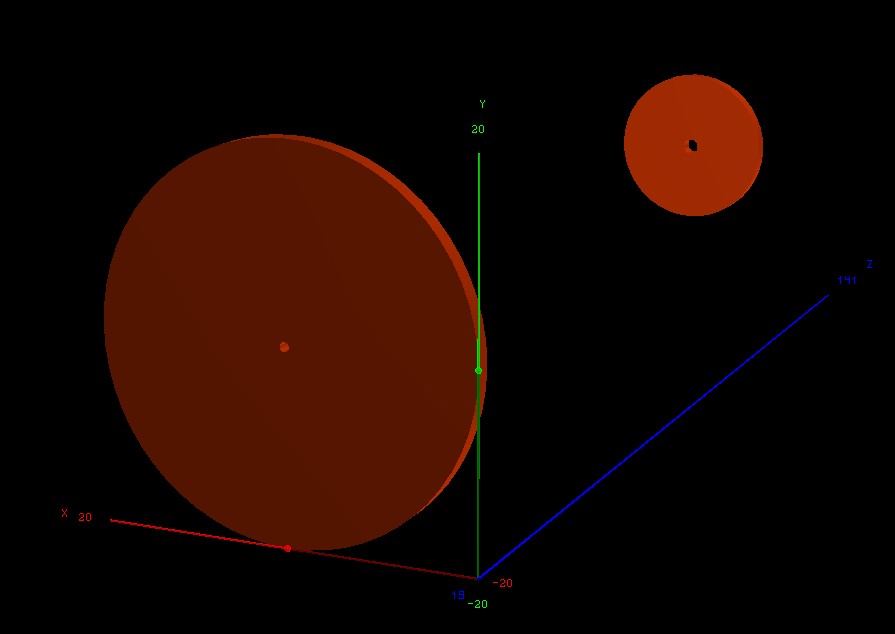
\includegraphics[width=0.77\textwidth]{img/gdml}
	\end{figure}
\end{frame}

\begin{frame}
	\ftitle
	\begin{block}{Example: Two quadrupoles}
		\texttt{<gpt>\\
			~~radius = 6e-3;\\
			~~setparticles("beam", 100, me, qe, 0.0);\\
			~~setrxydist("beam", "u", radius/2, radius);\\
			~~setphidist("beam", "u", 0, 2*pi);\\
			~~setGdist("beam", "u", 100, 0);\\
			~~quadrupole("wcs", "z", 0.2, 0.1,  3.90);\\
			~~quadrupole("wcs", "z", 0.5, 0.2, -3.25);\\
			~~G4Virtual("wcs", "i");\\
			~~tout(0, 4e-9, 0.05e-9);\\
			</gpt>
		}
	\end{block}
\end{frame}


\mysubsection{Output}

\begin{frame}
	\ftitle
	\begin{block}{Current outputs availible}
		\begin{itemize}
			\item GPT outputs (e.g. Divergence, Emittance, Standard deviations, ...)
			\item Trajectories (seperated by particle type, massless only here) as ASCII
			\item Dose and energy deposition in the geometry as ASCII
		\end{itemize}
	\end{block}
	\pause
	\begin{exampleblock}{Configuration of outputs}
		\texttt{<outputs>\\
			~~<output name="trajectories" />\\
			~~<output name="dose" x\_min="-1e3" x\_max="1e3"\\
			~~~~~~~~~~y\_min="-1e3" y\_max="1e3" z\_min="0" z\_max="2e3"\\
			~~~~~~~~~~nx="1000" ny="1000" nz="2000" />\\
			</outputs>
		}
	\end{exampleblock}
\end{frame}

\mysubsection{Optimization}

\begin{frame}
	\ftitle
	\begin{columns}
		\begin{column}{7cm}
			\begin{block}{Parallization of the \geant part}
				\begin{itemize}
					\item Single particles are independant
					\item \geant and output distributed over several threads using OpenMP (previous versions also MPI)
					\item Configurable with environment variables
				\end{itemize}
			\end{block}
			\pause
			\begin{exampleblock}{Other optimizations}
				There are additional optimizations, e.g. for output, particle exchange, ...
			\end{exampleblock}
		\end{column}
		\begin{column}{4cm}
			\begin{figure}
				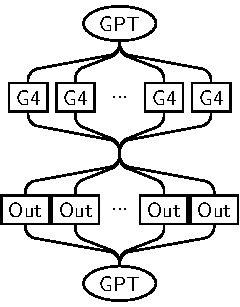
\includegraphics[width=\columnwidth]{img/parallel_flow}
			\end{figure}
		\end{column}
	\end{columns}
\end{frame}


\section{Verification and applications}

\mysubsection{Comparison to pure GPT}

\begin{frame}
	\ftitle
	\begin{columns}
		\begin{column}{7.1cm}
			\begin{block}{The quadrupole example}
				\begin{itemize}
					\item Basically the same world as in a GPT example: Two quadrupoles ($G = 3.9, -3.25 ~\frac{T}{m}$) focus a beam of electrons ($\gamma = 100$)
					\item Empty space filled with weak interacting gas ($H_2$), two pinholes ($Cu$)
					\item Possibility to test the stepping algorithm
				\end{itemize}
			\end{block}
			\pause
			\begin{exampleblock}{The result}
				Flint and GPT both focus at $z = 1.3~m$
			\end{exampleblock}
		\end{column}
		\begin{column}{4cm}
			\begin{figure}
				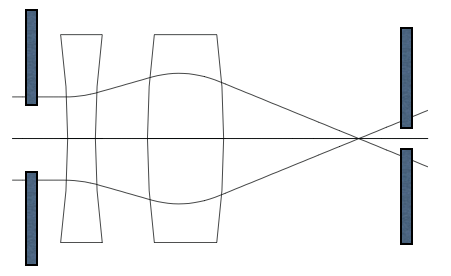
\includegraphics[width=\columnwidth]{img/quadrupole_setup}\\\vskip 12pt
				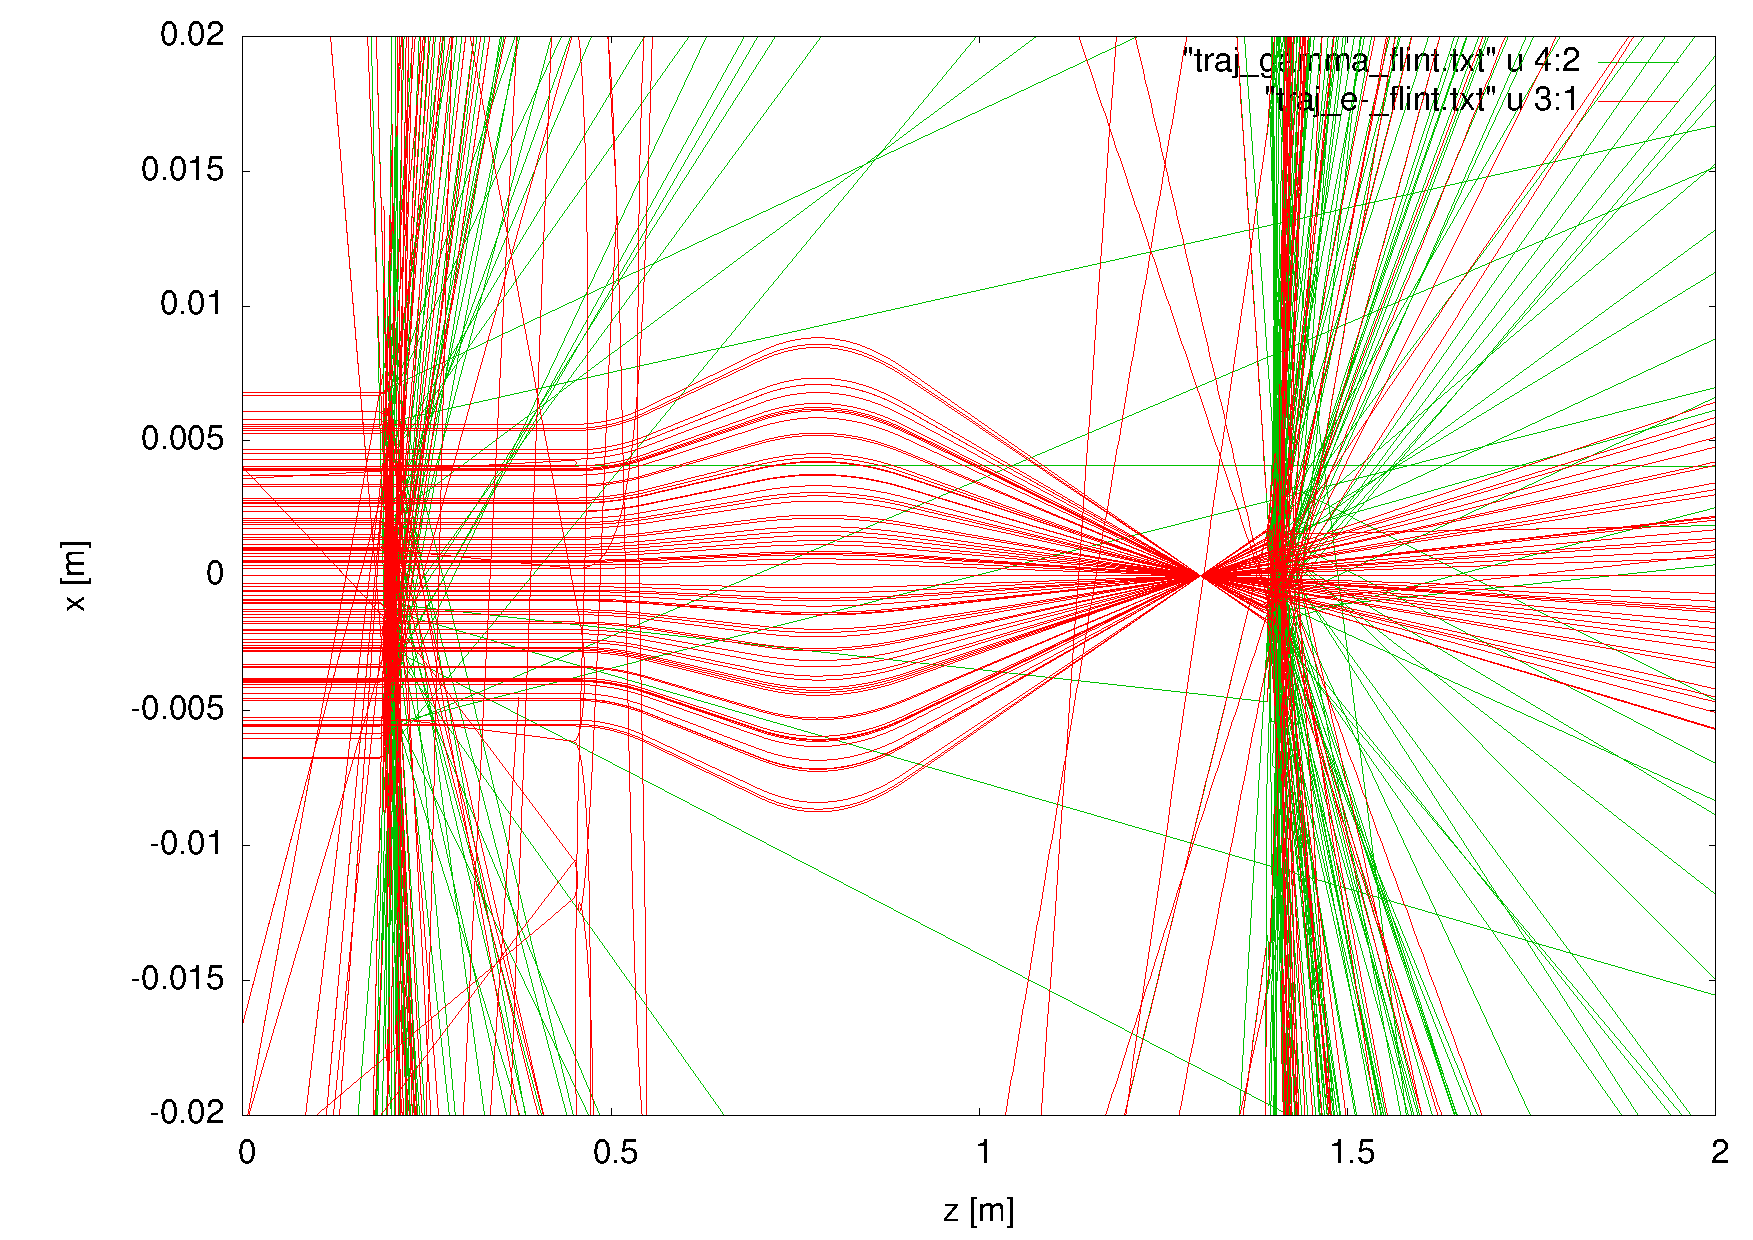
\includegraphics[width=\columnwidth]{img/quadrupole_flint}
			\end{figure}
		\end{column}
	\end{columns}
\end{frame}

\begin{frame}
	\ftitle
	\begin{figure}
		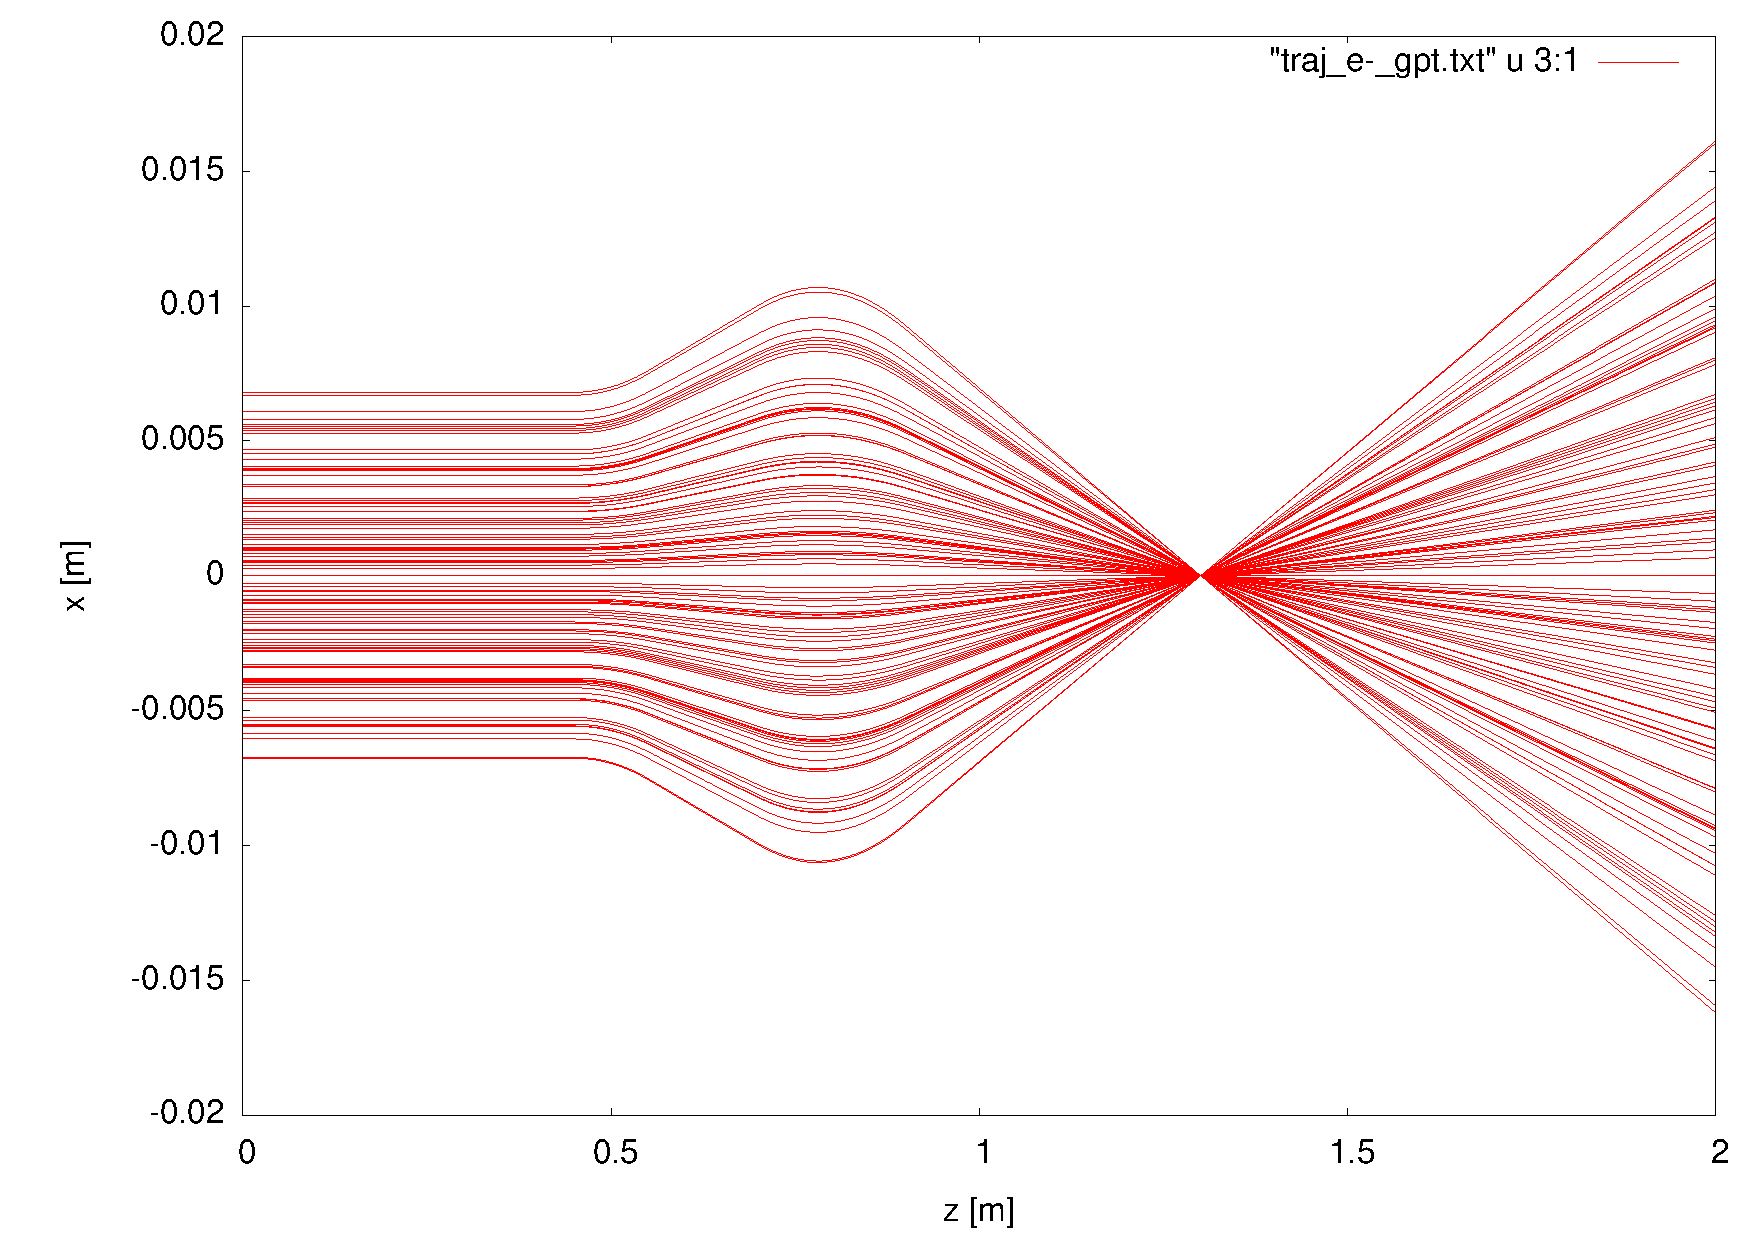
\includegraphics[height=0.8\textheight]{img/quadrupole_gpt}
	\end{figure}
\end{frame}

\begin{frame}
	\ftitle
	\begin{figure}
		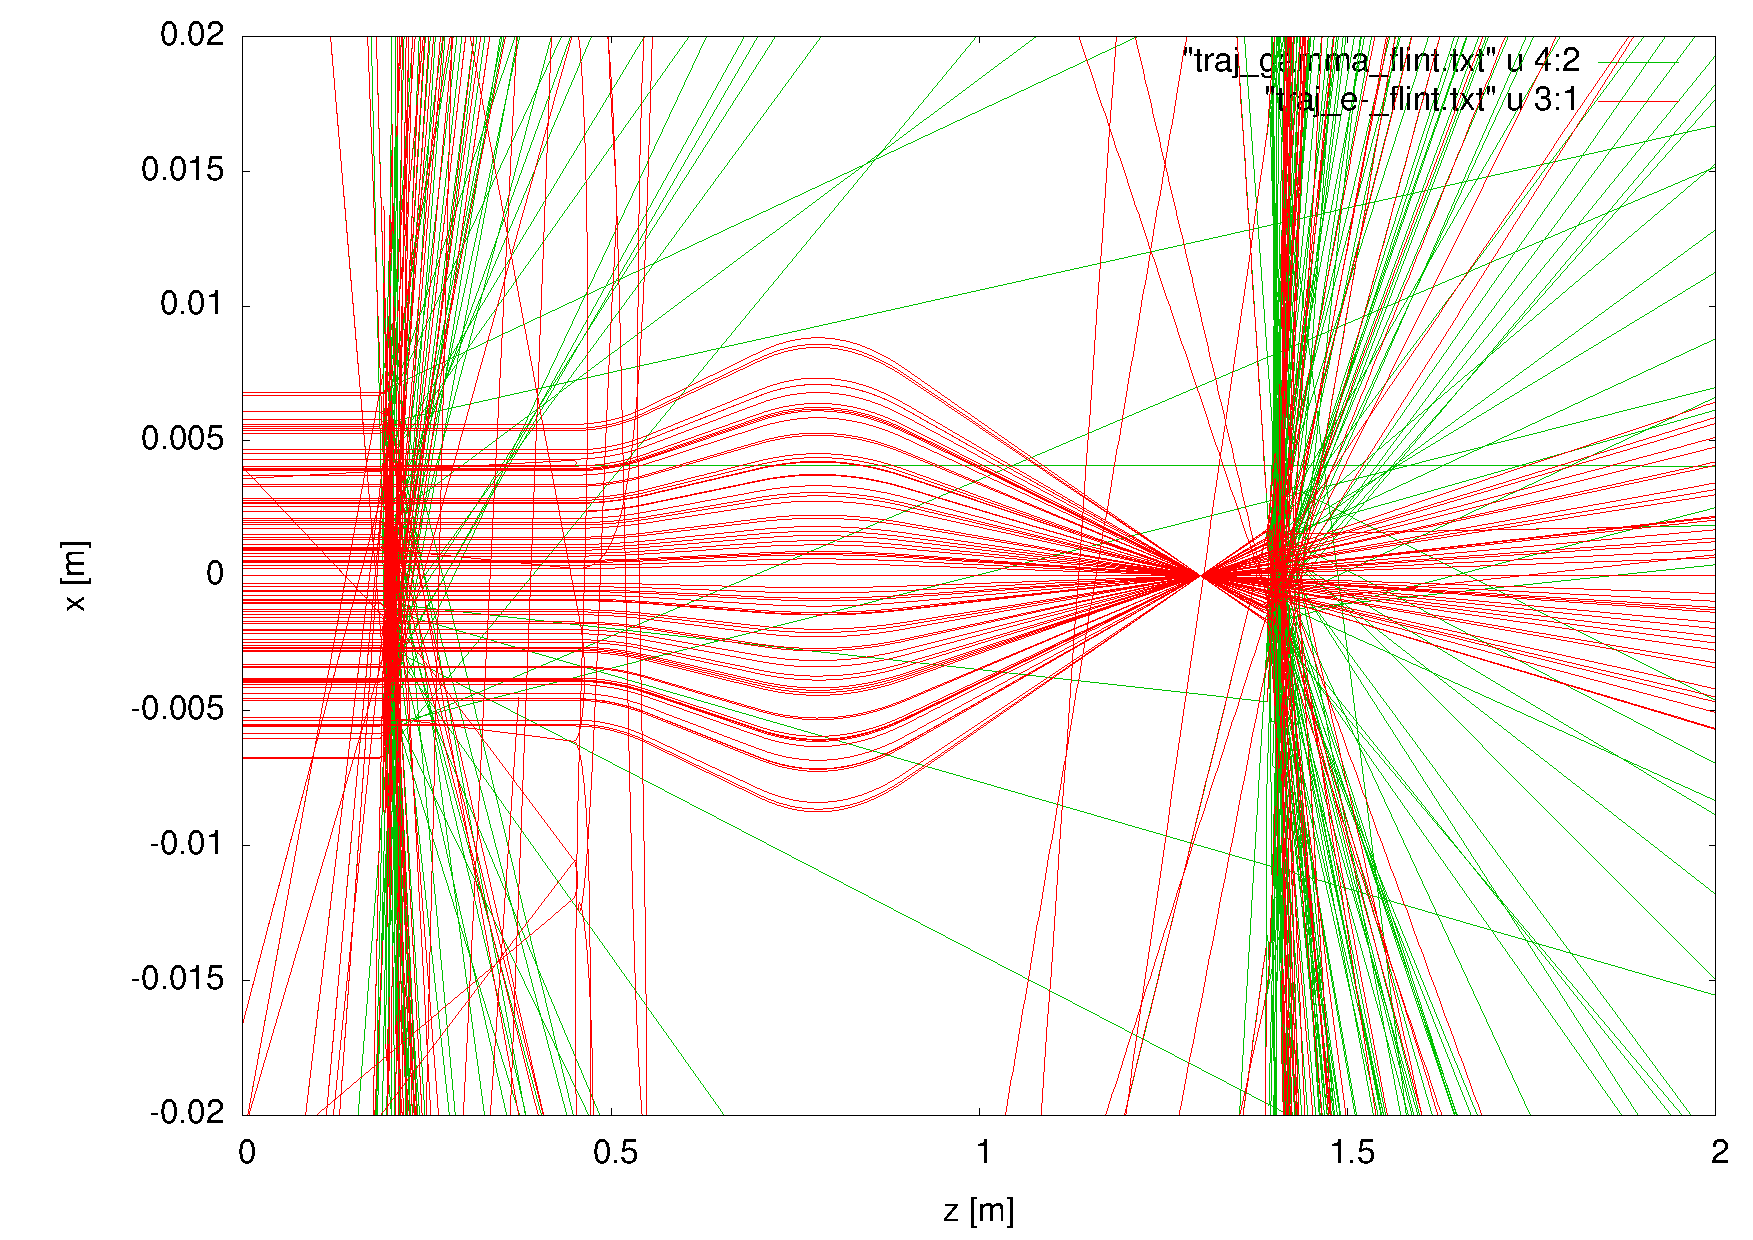
\includegraphics[height=0.8\textheight]{img/quadrupole_flint}
	\end{figure}
\end{frame}

\begin{frame}
	\ftitle
	\begin{figure}
		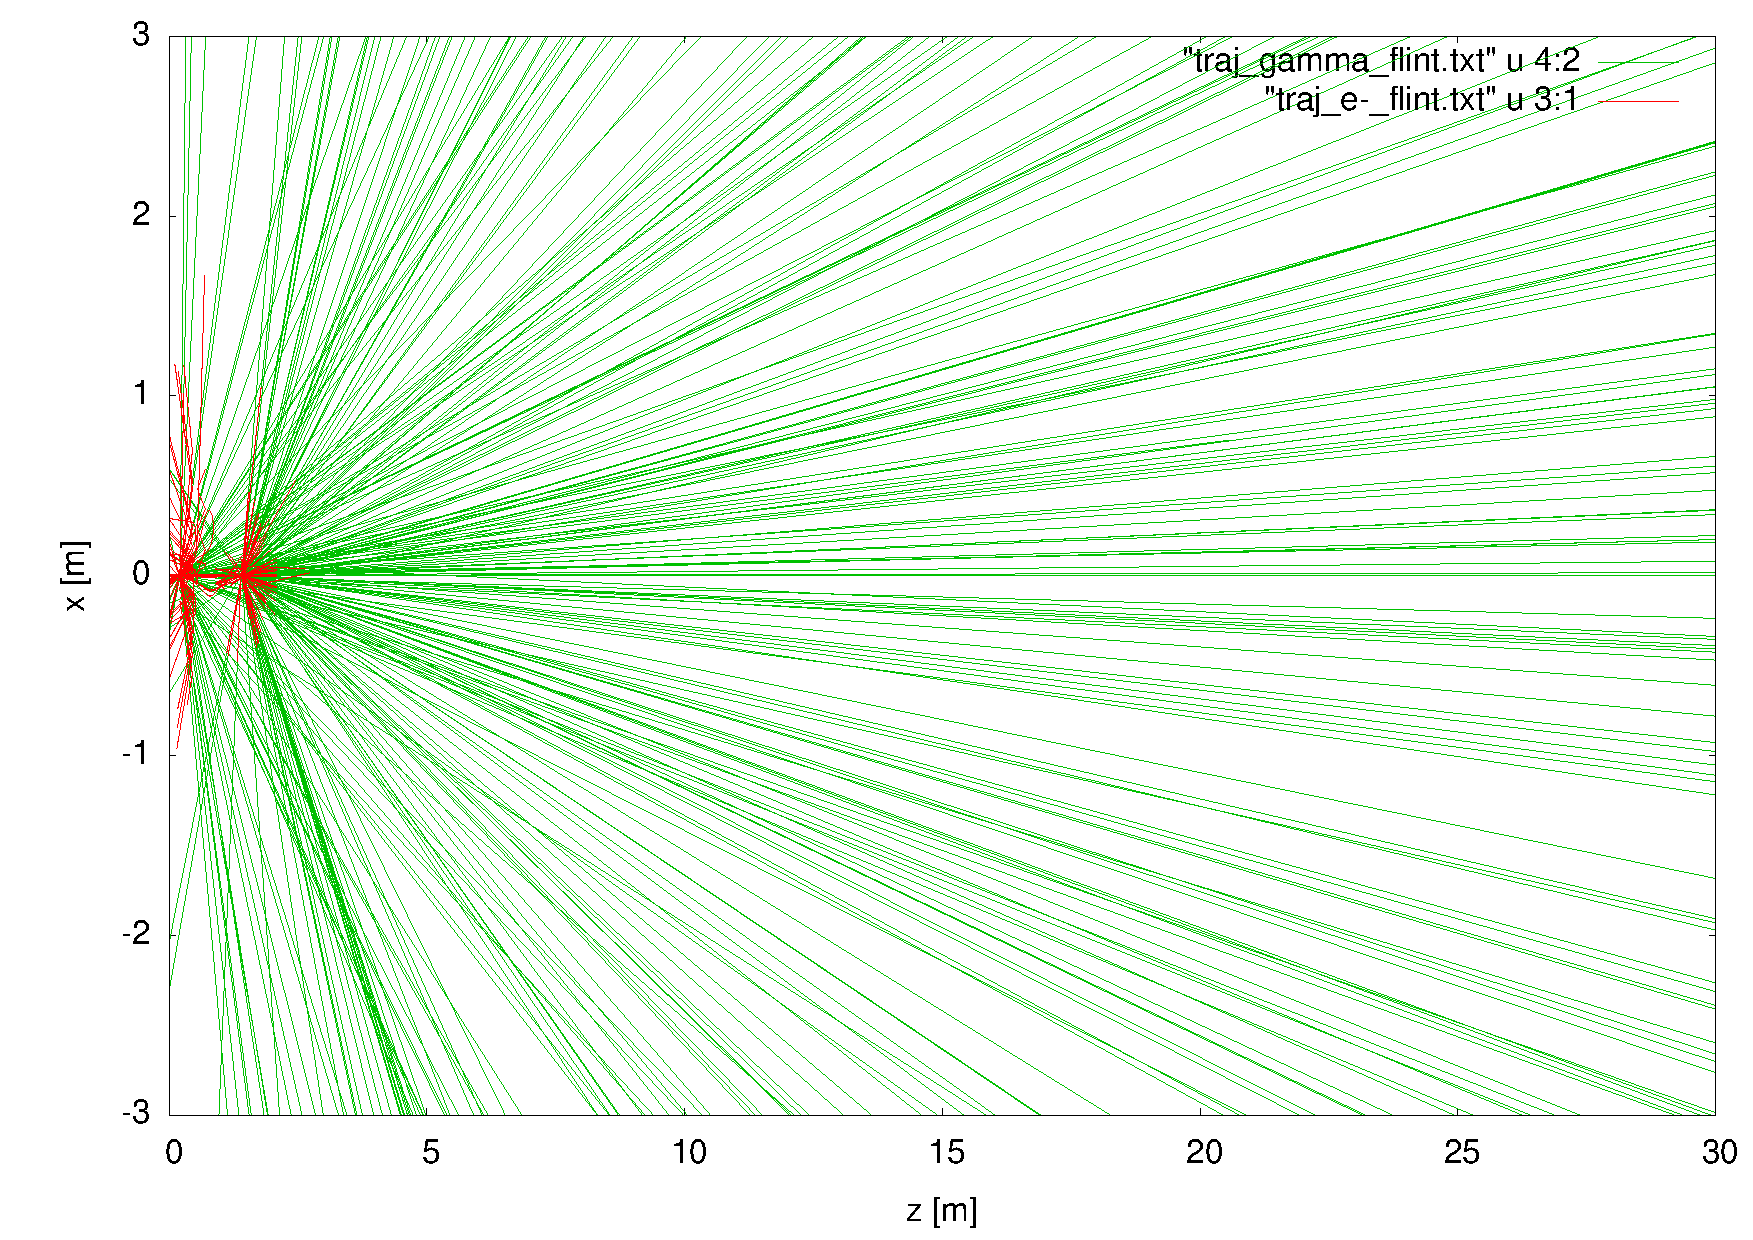
\includegraphics[height=0.8\textheight]{img/quadrupole_gamma}
	\end{figure}
\end{frame}

\mysubsection{Comparison to pure \geant}

\begin{frame}
	\ftitle
	\begin{columns}
		\begin{column}{7.5cm}
			\begin{block}{Emittance calculation}
				\begin{itemize}
					\item Electron-beam with a Gaussian space-distribution with $\sigma = 0.3 ~\text{mm}$, $\varepsilon_0 = 1~ \text{mm}~\text{mrad}$, divergence of $190~\mu \text{rad}$, $\gamma = 440$
					\item Emittance after a thin ($d = (1, 4, 15) ~\mu\text{m}$) aluminium foil is compared to \geant
				\end{itemize}
			\end{block}
			\begin{exampleblock}<2->{The result}
				Both, Flint and \geantws, produce the same change in emittance (for $15~\mu\text{m}$ $Al$): $\varepsilon_0 = 81~\text{mm}~\text{mrad}$.
			\end{exampleblock}
		\end{column}
		\begin{column}{4cm}
			\begin{figure}
				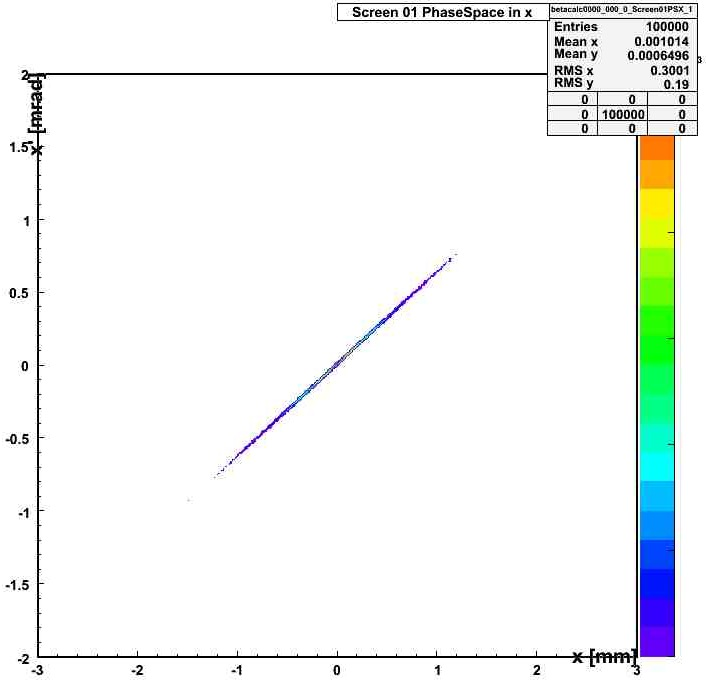
\includegraphics[width=0.67\columnwidth]{img/emittance_ps_pre}\\\vskip 10pt
				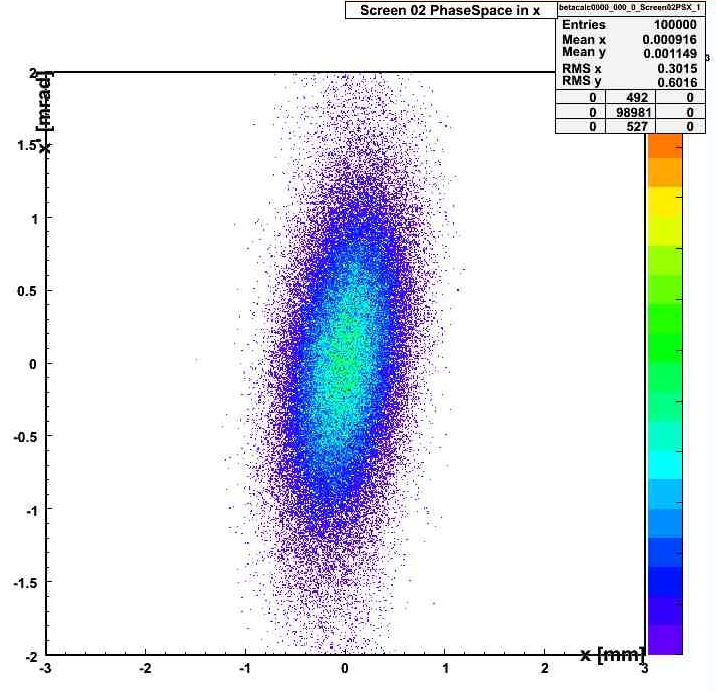
\includegraphics[width=0.67\columnwidth]{img/emittance_ps_post}
				\caption{Phase space}
			\end{figure}
		\end{column}
	\end{columns}
\end{frame}

\mysubsection{Design of a sample beamline}

\begin{frame}
	\ftitle
	\begin{columns}
		\begin{column}{6cm}
			\begin{block}{Designing a sample beamline}
				\begin{itemize}
					\item Beam: electrons ($\gamma = 100$) and protons ($\gamma = 5$)
					\item A pinhole (Cu)
					\item A separating magnetic field ($B = 2~T$)
					\item Protons collide into a beam dump (Pb)
				\end{itemize}
			\end{block}
		\end{column}
		\begin{column}{5cm}
			\begin{figure}
				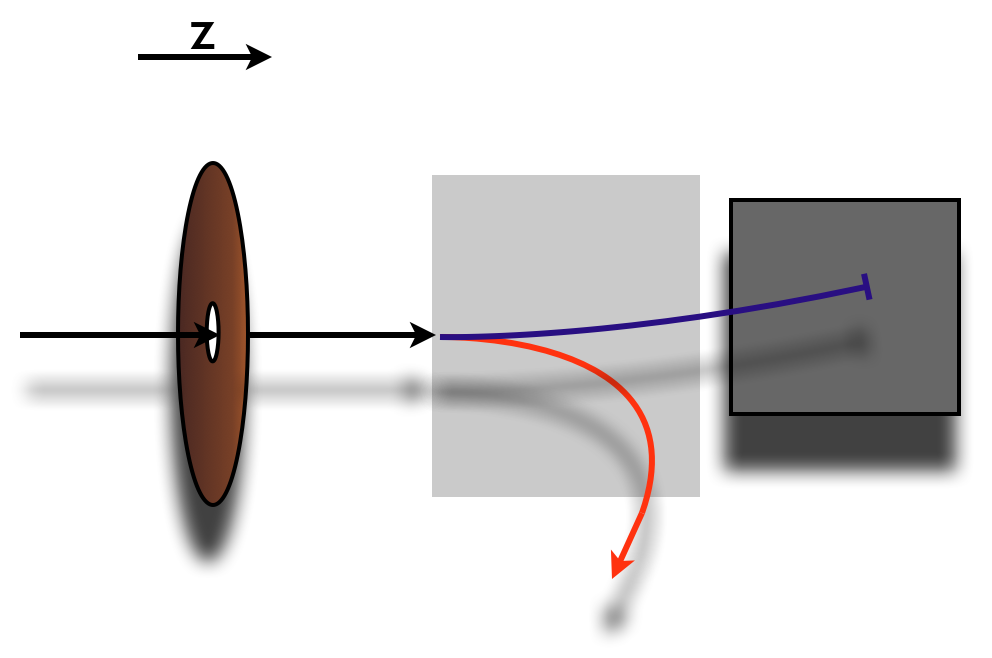
\includegraphics[width=\columnwidth]{img/beamline_setup}
			\end{figure}
		\end{column}
	\end{columns}
\end{frame}

\begin{frame}
	\ftitle
	\begin{figure}
		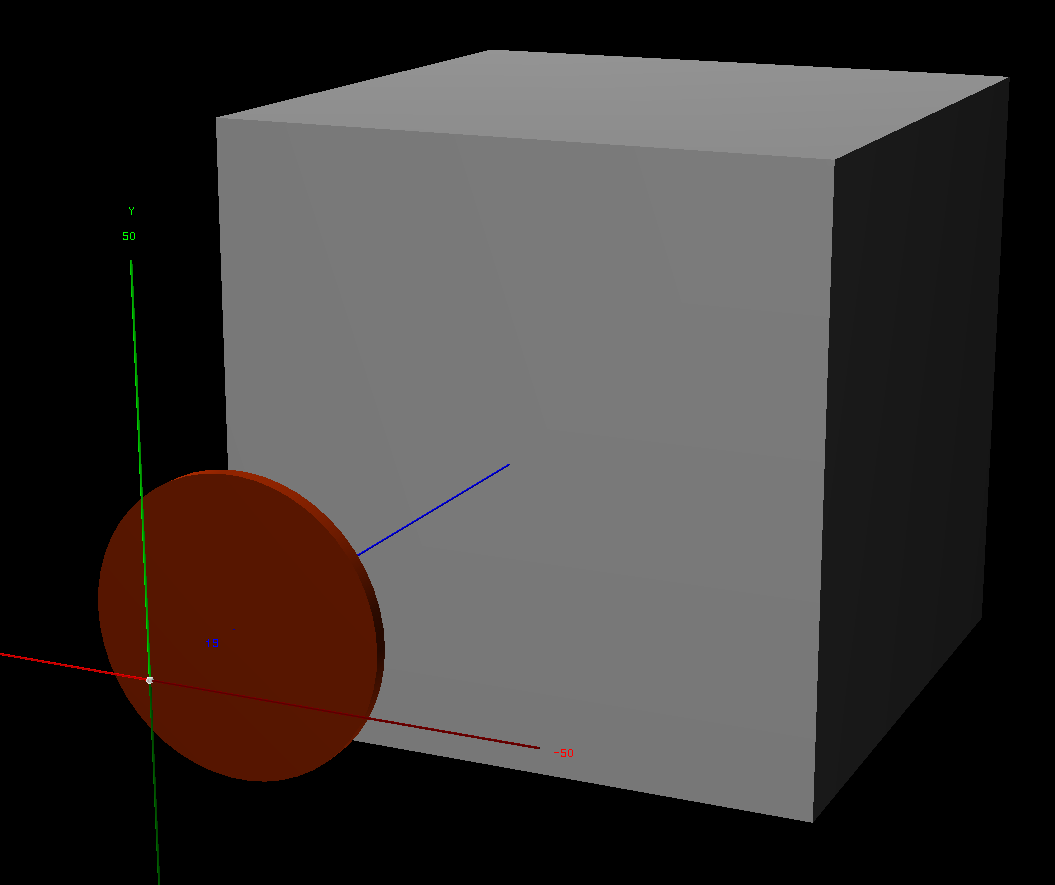
\includegraphics[width=0.65\textwidth]{img/beamline_setup_3d}
	\end{figure}
\end{frame}

\begin{frame}
	\ftitle
	\begin{figure}
		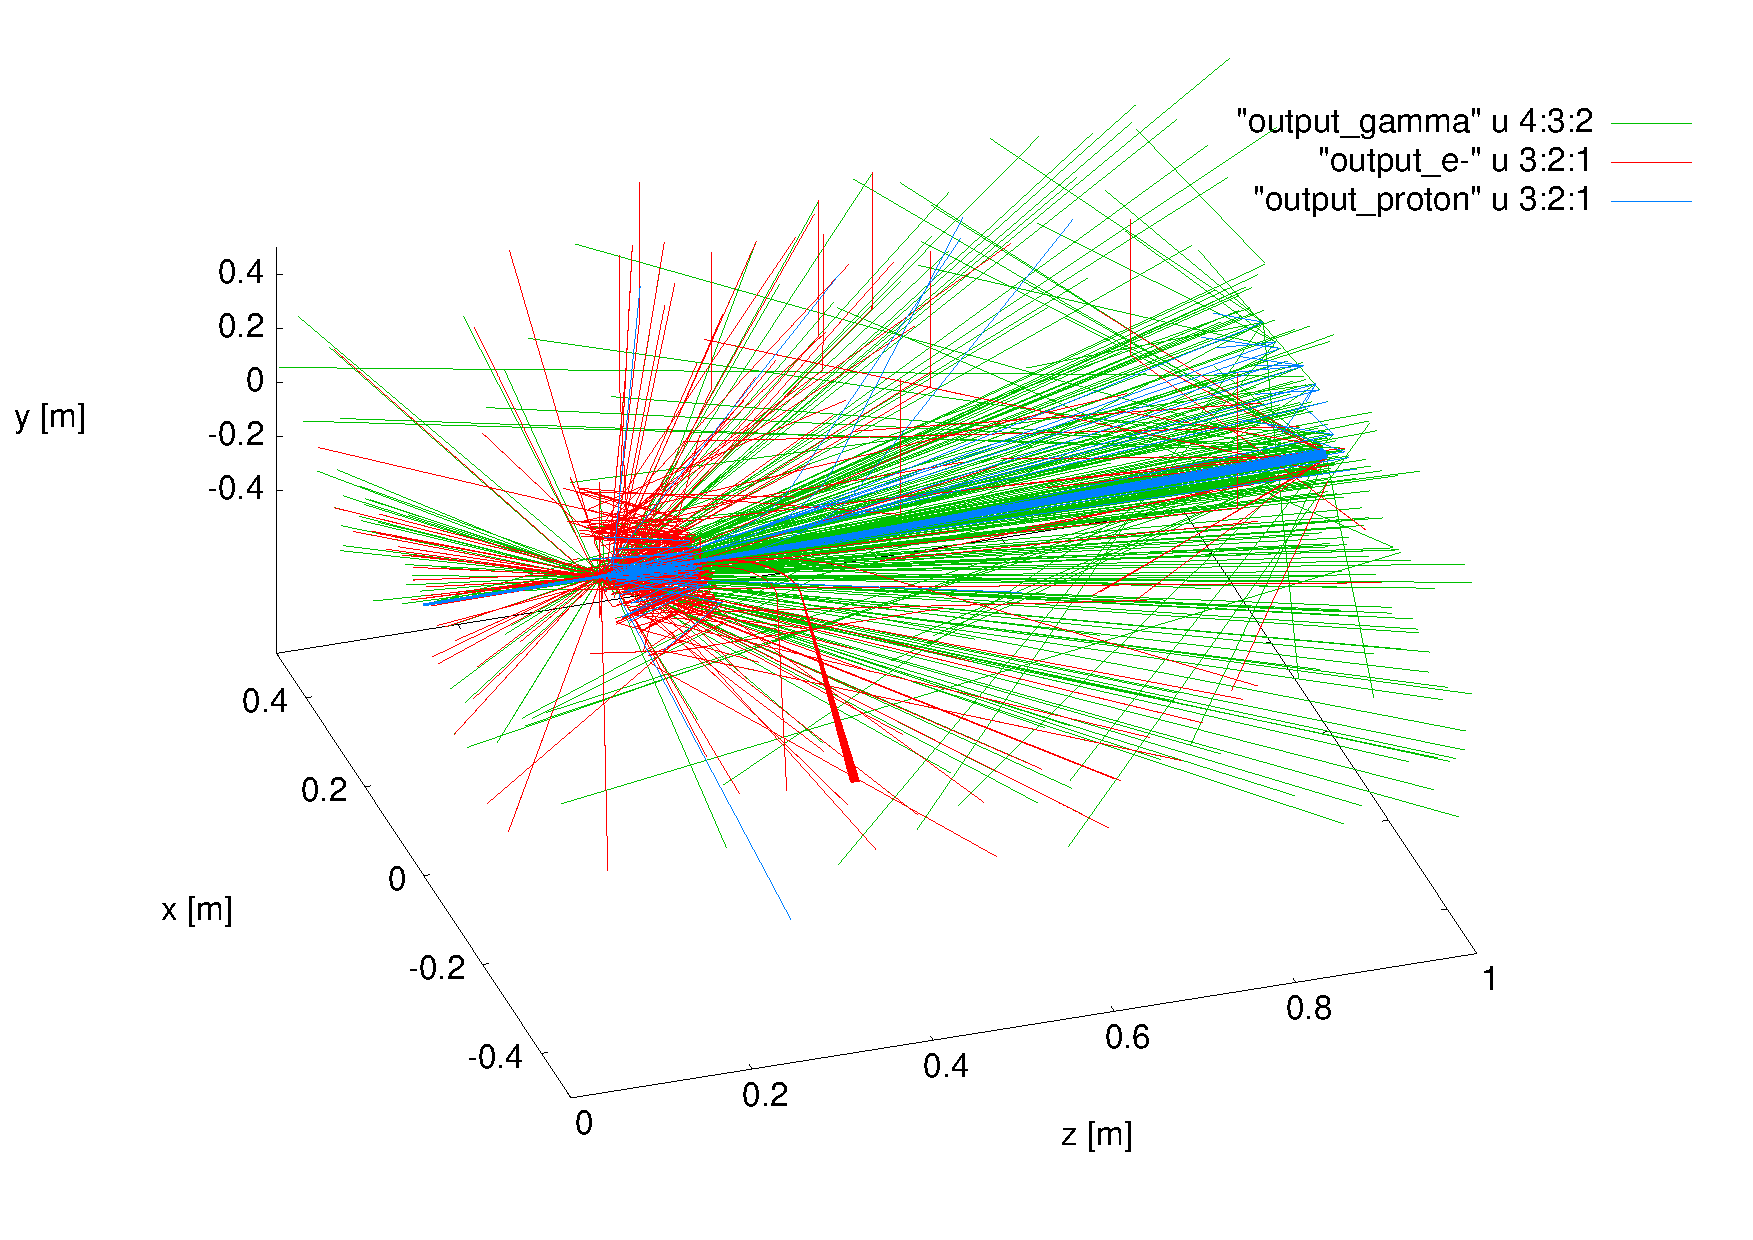
\includegraphics[width=0.7\textwidth]{img/beamline_traj_3d}
		\caption{Also produced: $\alpha$, $e^+$, neutrons}
	\end{figure}
\end{frame}

\begin{frame}
	\ftitle
	\begin{figure}
		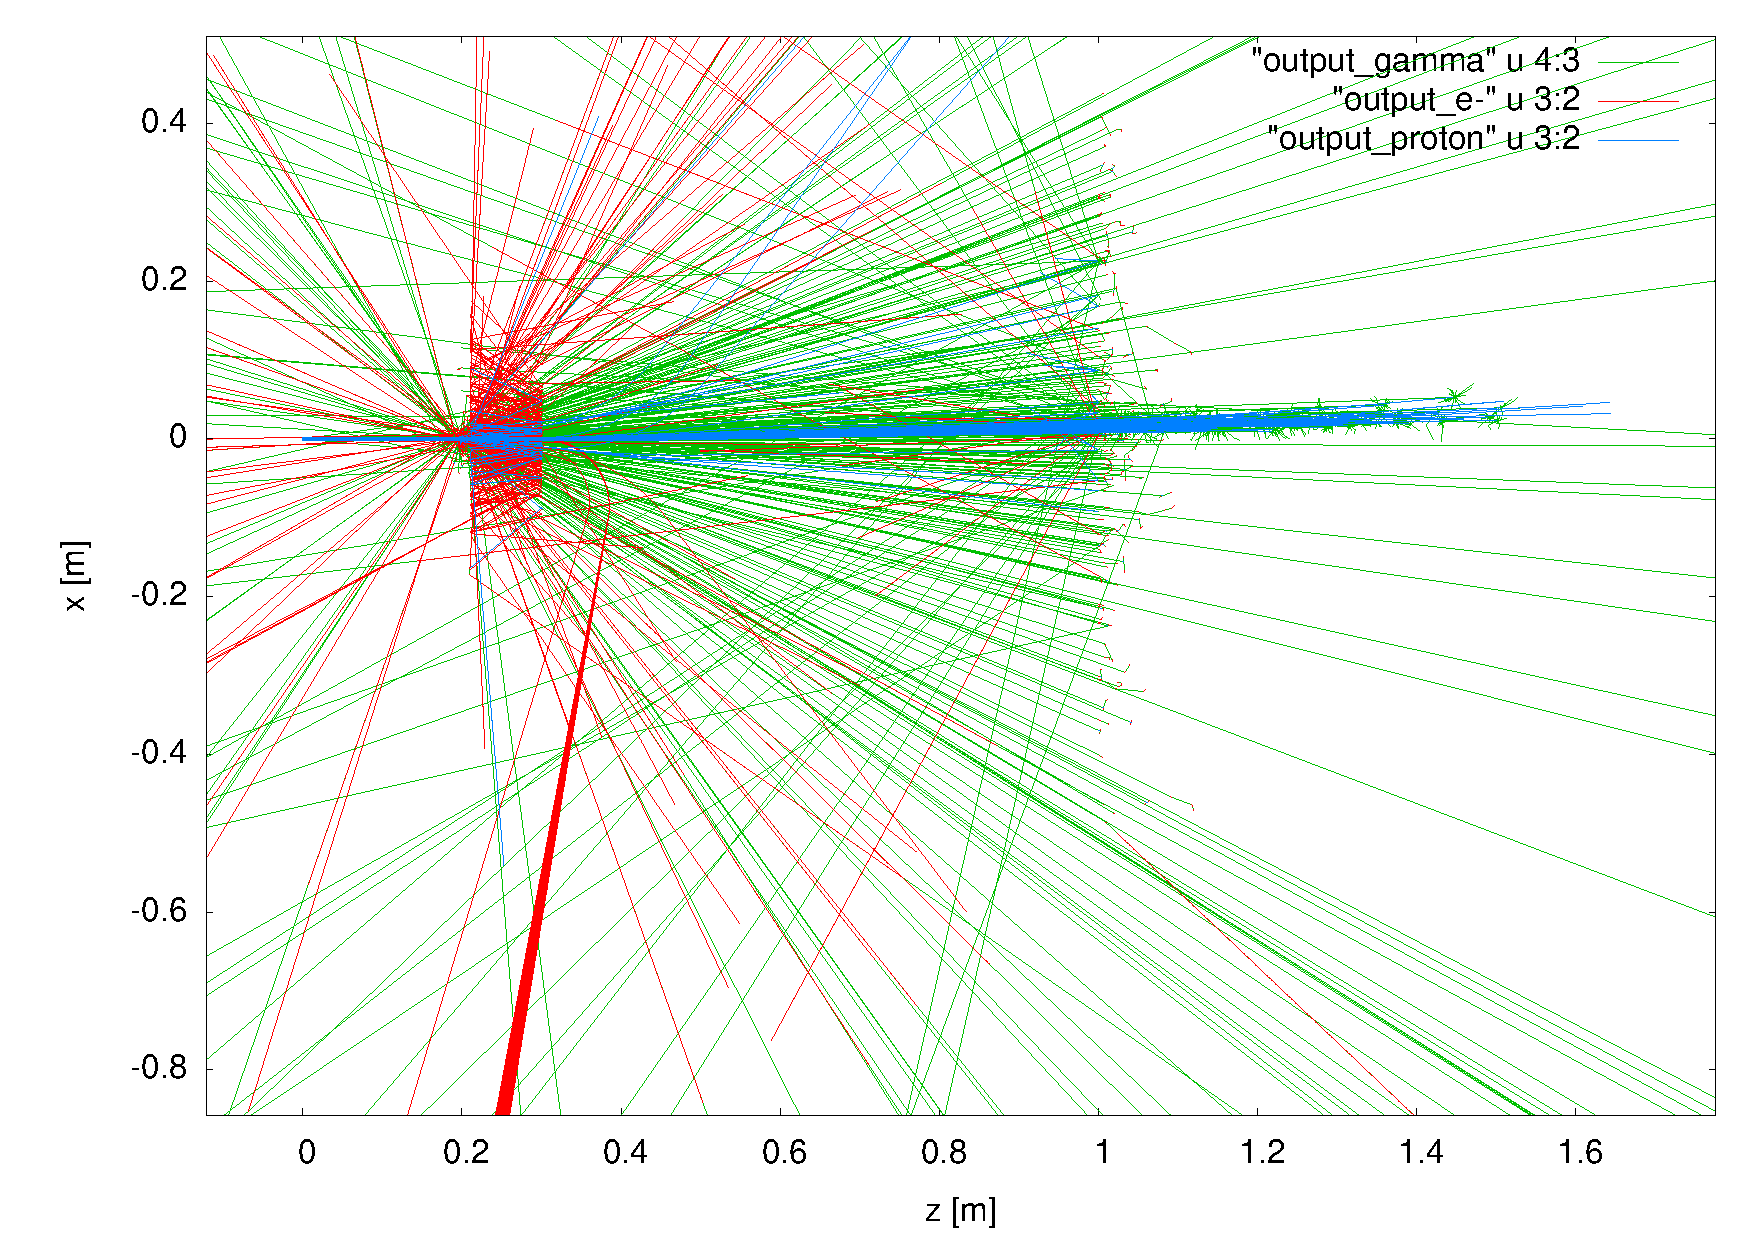
\includegraphics[width=0.75\textwidth]{img/beamline_traj_overview}~
		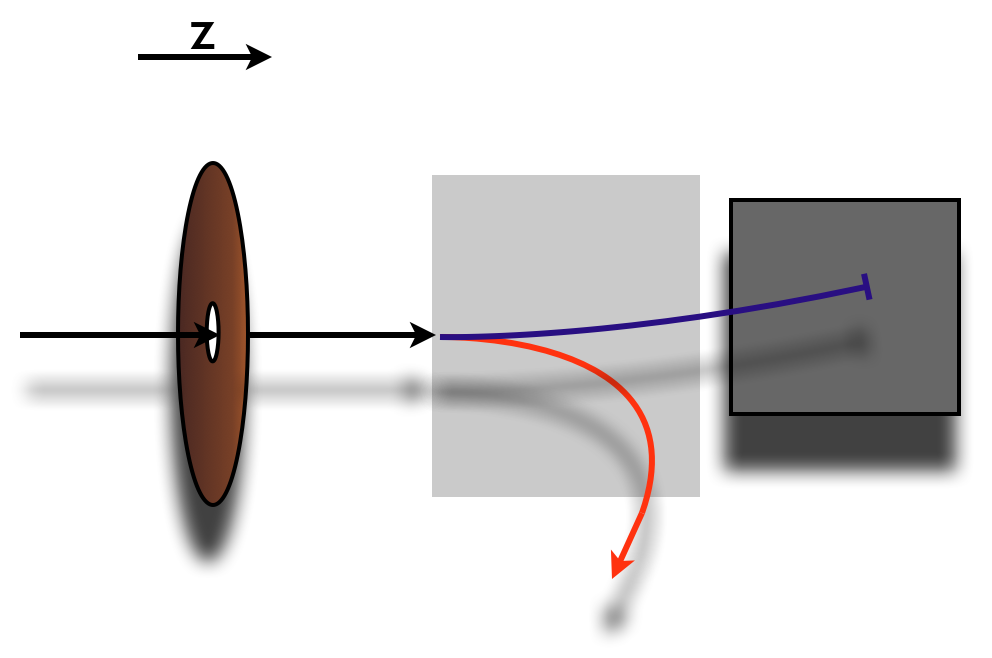
\includegraphics[width=0.25\textwidth]{img/beamline_setup}
	\end{figure}
\end{frame}

\begin{frame}
	\ftitle
	\begin{figure}
		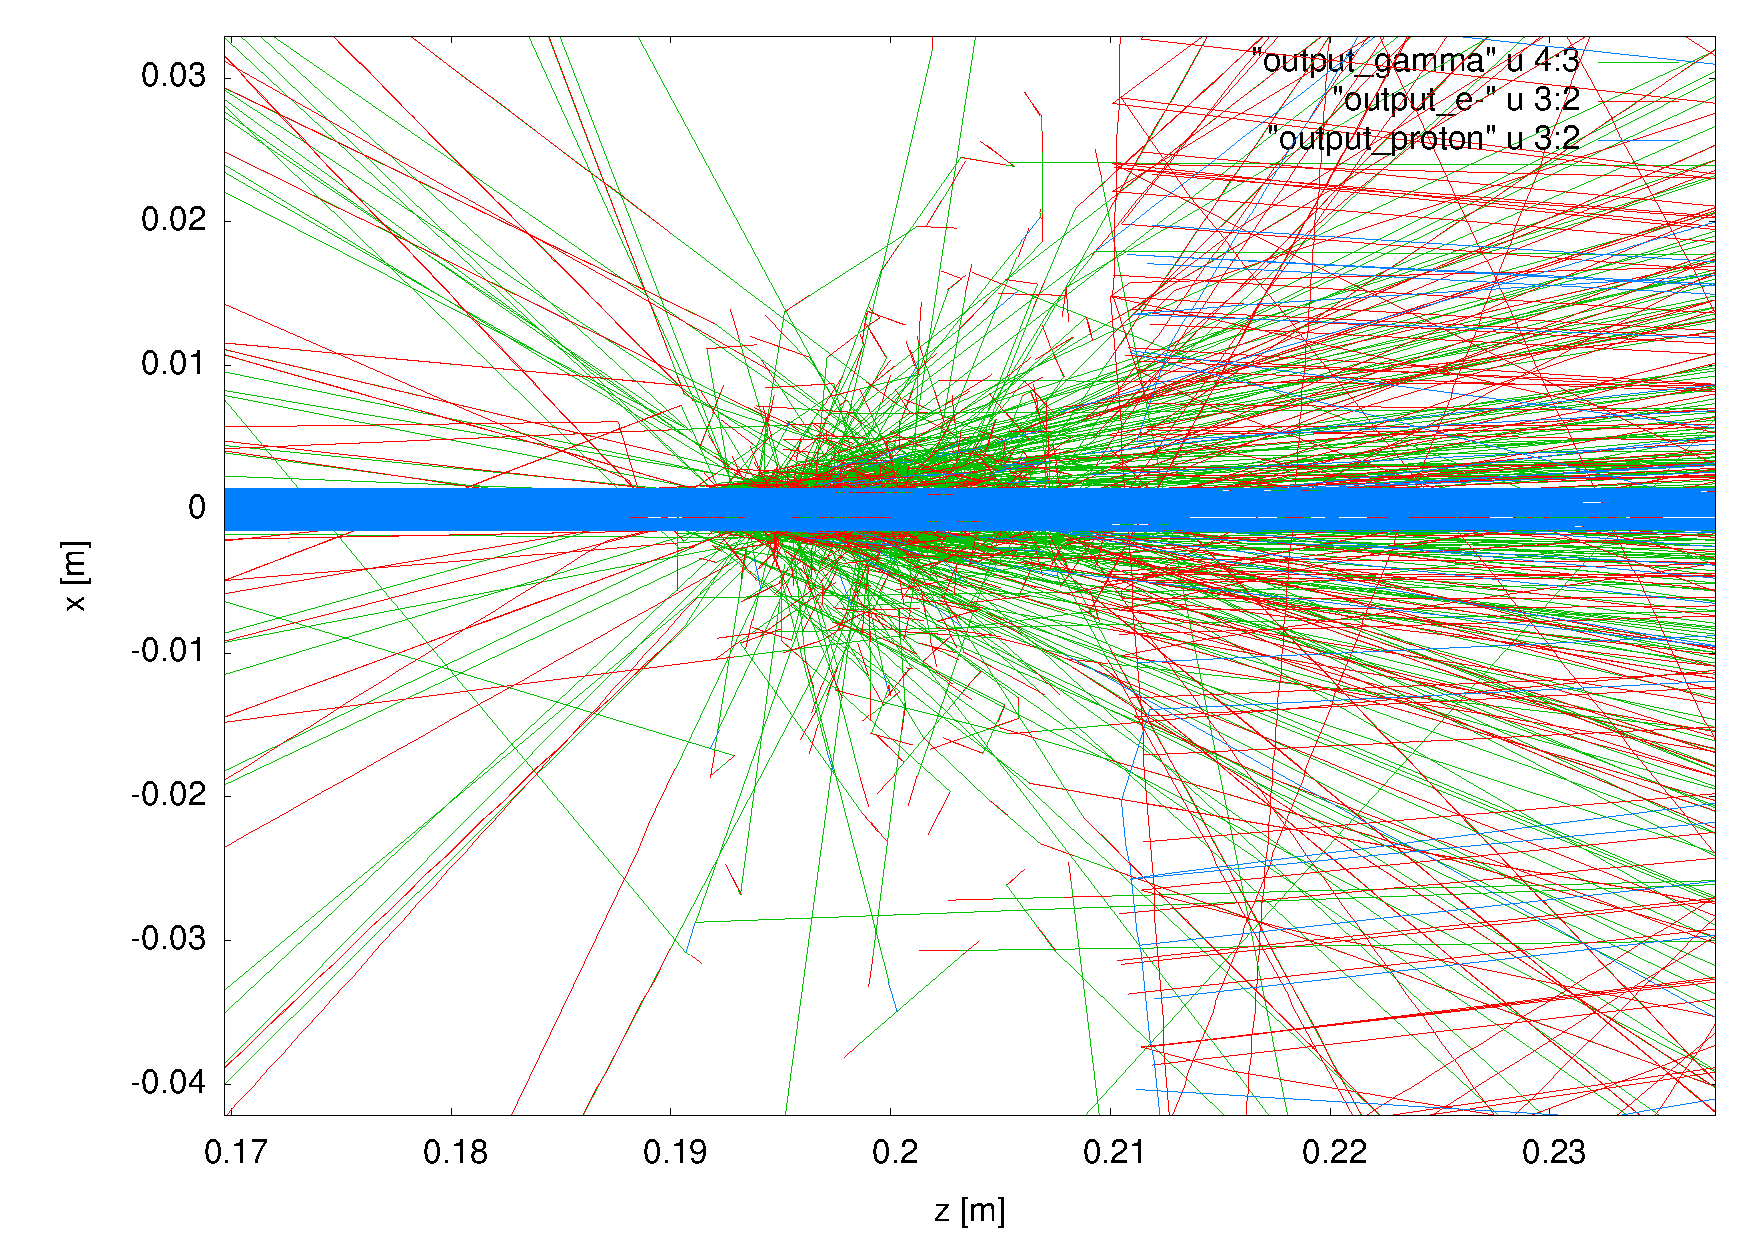
\includegraphics[width=0.8\textwidth]{img/beamline_traj_pinhole}
	\end{figure}
\end{frame}

\begin{frame}
	\ftitle
	\begin{figure}
		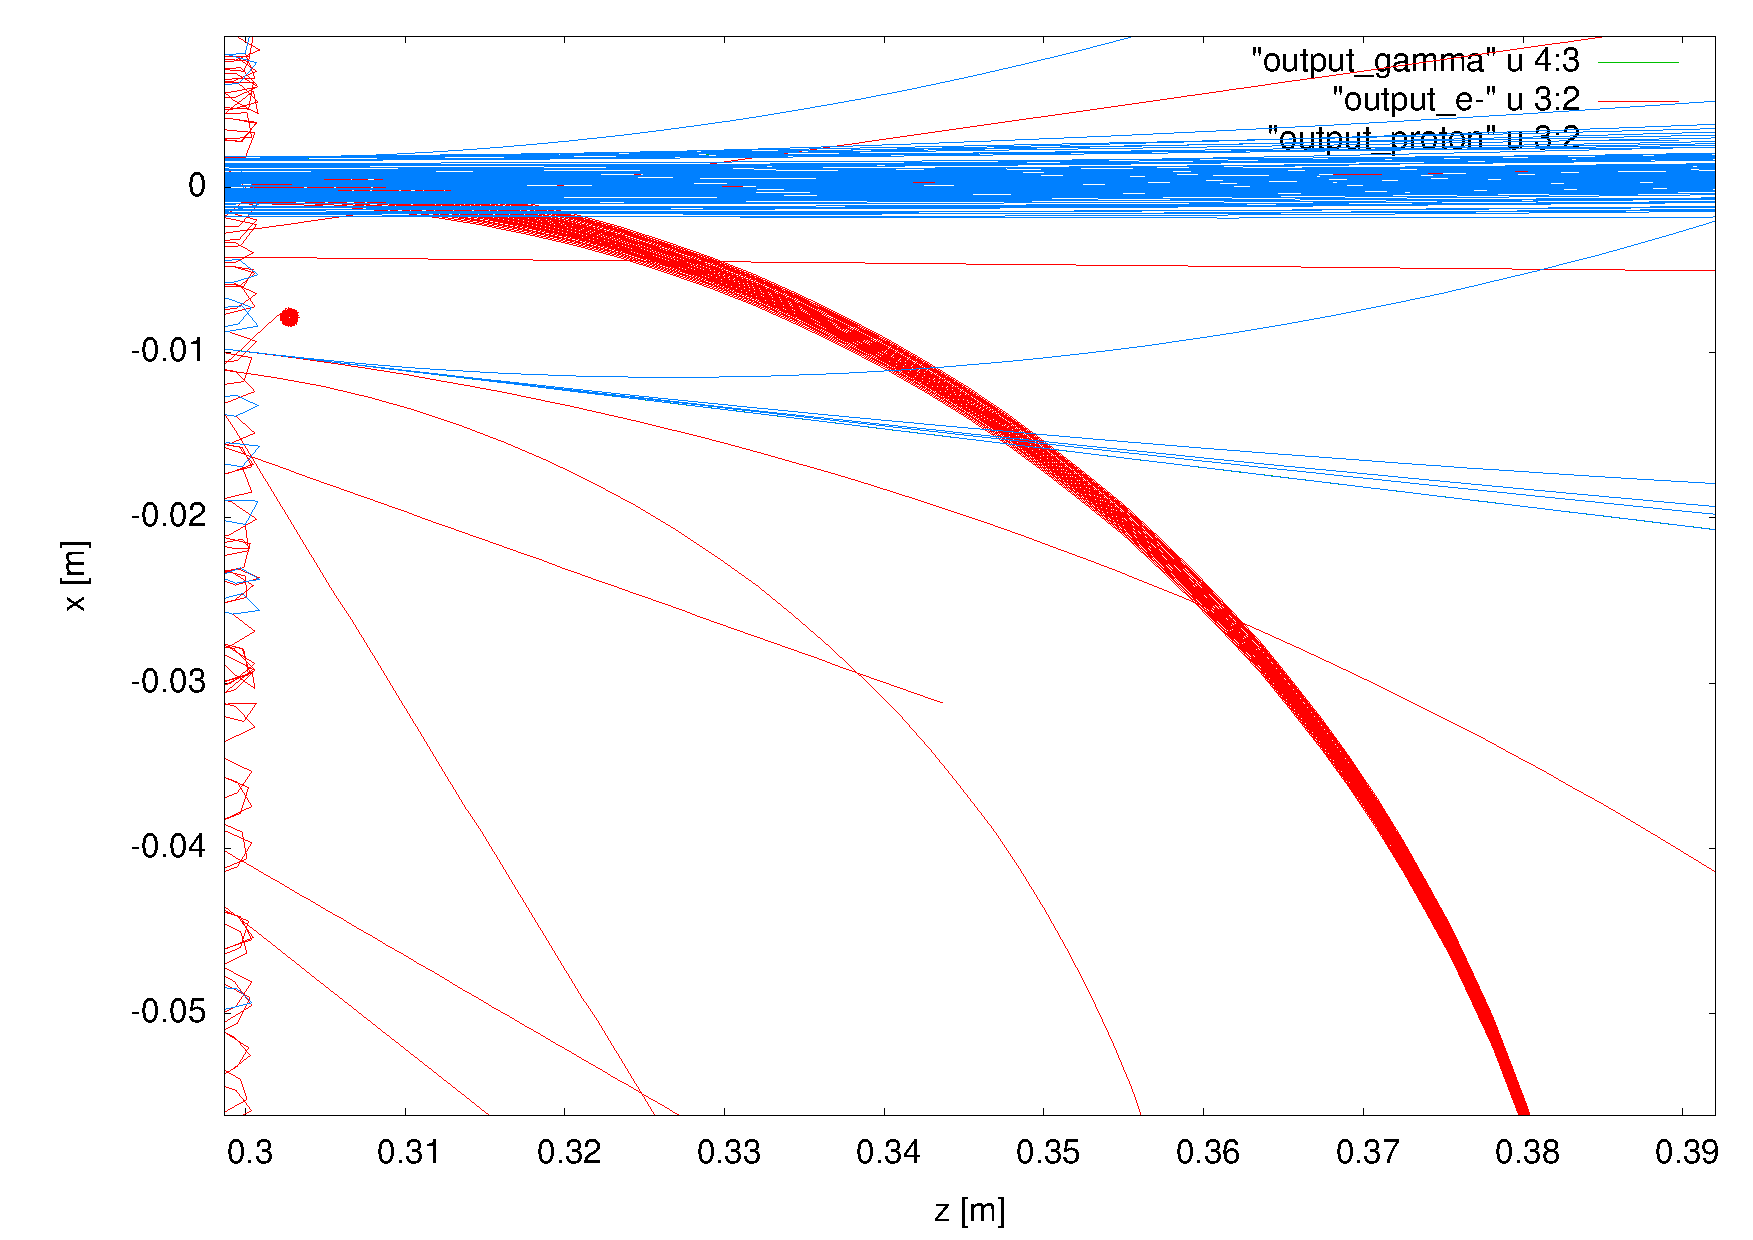
\includegraphics[width=0.8\textwidth]{img/beamline_traj_spectrometer}
	\end{figure}
\end{frame}

\begin{frame}
	\ftitle
	\begin{figure}
		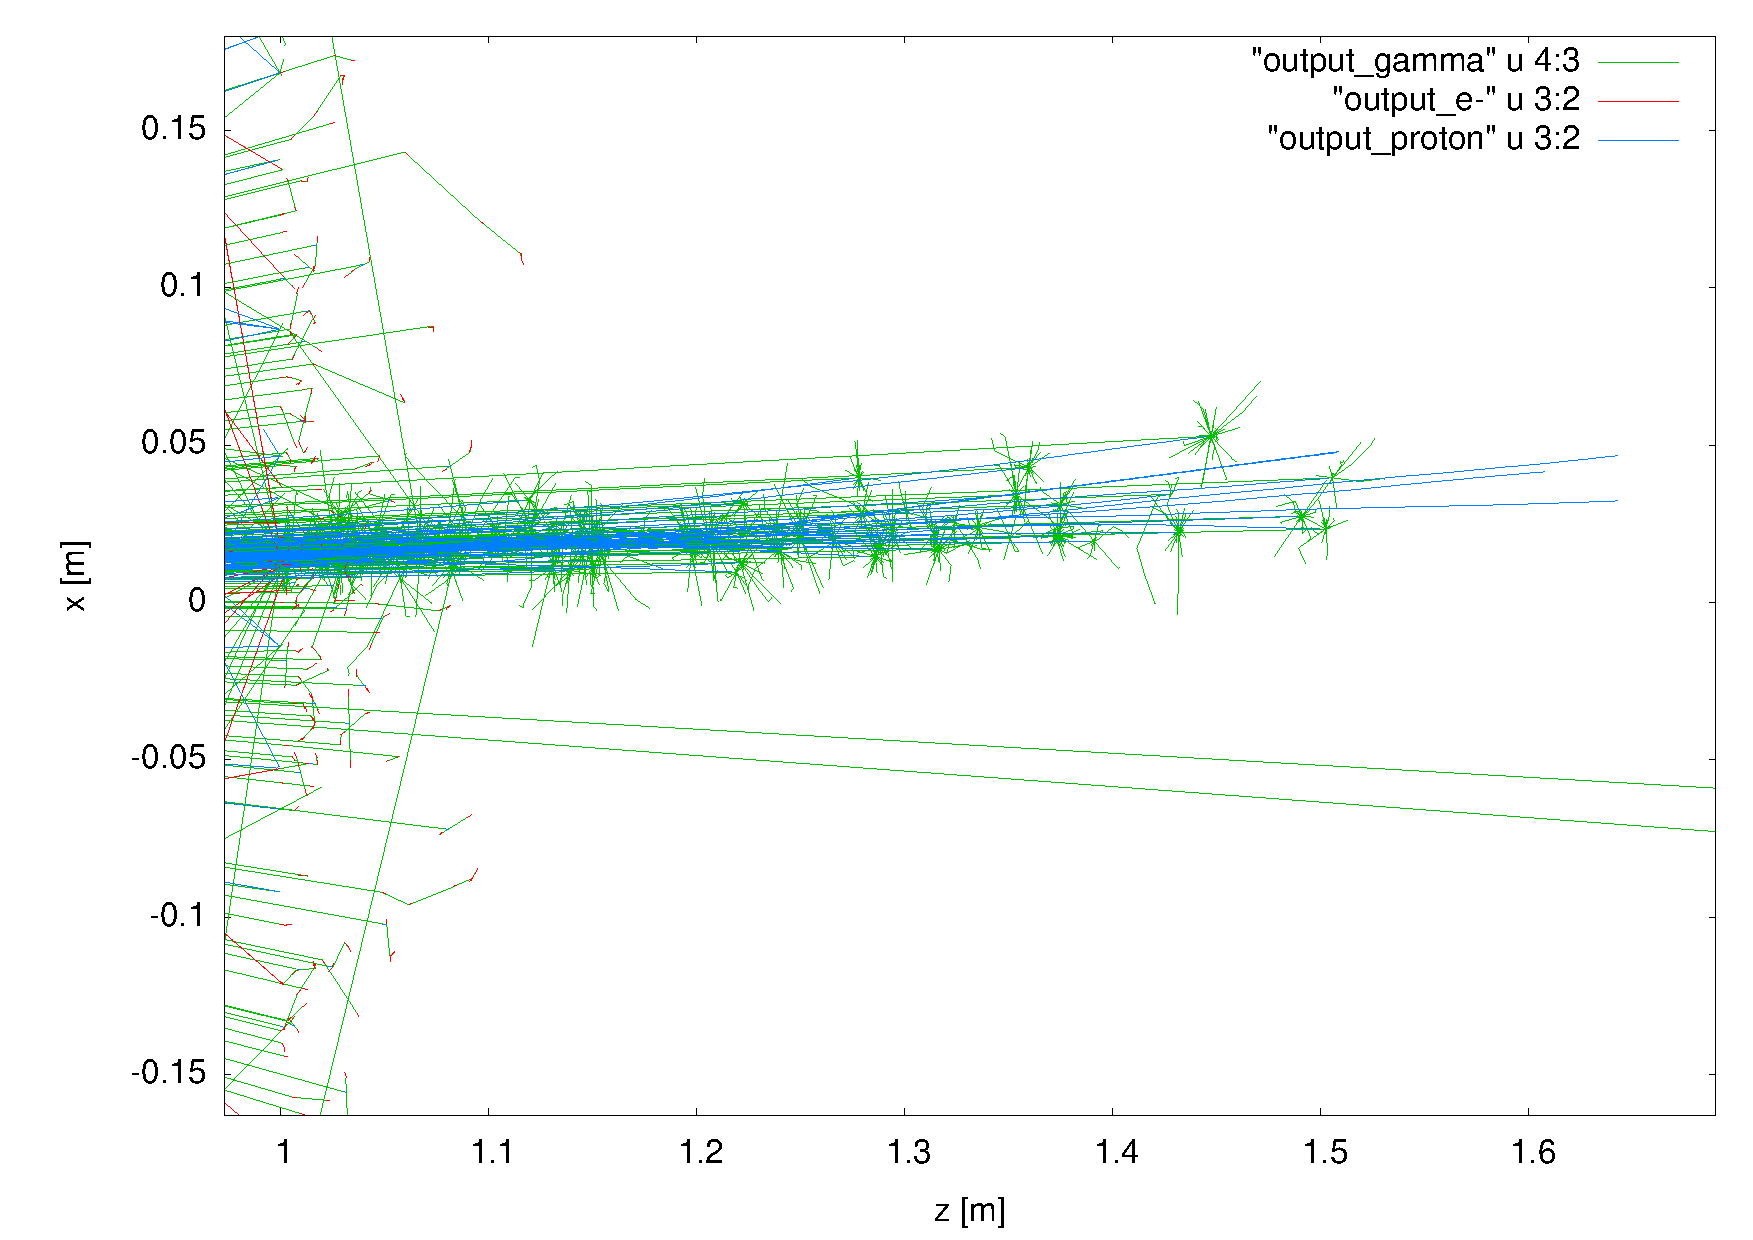
\includegraphics[width=0.8\textwidth]{img/beamline_traj_beamdump}
	\end{figure}
\end{frame}

\mysubsection{Outlook}

\begin{frame}
	\ftitle
	\begin{block}{Software impropvements}
		\begin{itemize}
			\item Some minor and major optimizations
			\item More configurability through XML (perhaps replace GPT \texttt{ini} file)
		\end{itemize}
	\end{block}
	\pause
	\begin{exampleblock}{Major improvements}
		\begin{itemize}
			\item Use \geantws's proposed step length in GPT
			\item More output options (e.g. detailed interaction information)
			\item Use another format than ASCII for output (speedup)
			\item More testing (e.g. tracking ions, fission processes, complex space charge effects)
		\end{itemize}
	\end{exampleblock}
\end{frame}

\end{document}
